\documentclass[twoside]{article}

% Packages required by doxygen
\usepackage{fixltx2e}
\usepackage{calc}
\usepackage{doxygen}
\usepackage[export]{adjustbox} % also loads graphicx
\usepackage{graphicx}
\usepackage[utf8]{inputenc}
\usepackage{makeidx}
\usepackage{multicol}
\usepackage{multirow}
\PassOptionsToPackage{warn}{textcomp}
\usepackage{textcomp}
\usepackage[nointegrals]{wasysym}
\usepackage[table]{xcolor}

% Font selection
\usepackage[T1]{fontenc}
\usepackage[scaled=.90]{helvet}
\usepackage{courier}
\usepackage{amssymb}
\usepackage{sectsty}
\renewcommand{\familydefault}{\sfdefault}
\allsectionsfont{%
  \fontseries{bc}\selectfont%
  \color{darkgray}%
}
\renewcommand{\DoxyLabelFont}{%
  \fontseries{bc}\selectfont%
  \color{darkgray}%
}
\newcommand{\+}{\discretionary{\mbox{\scriptsize$\hookleftarrow$}}{}{}}

% Page & text layout
\usepackage{geometry}
\geometry{%
  a4paper,%
  top=2.5cm,%
  bottom=2.5cm,%
  left=2.5cm,%
  right=2.5cm%
}
\tolerance=750
\hfuzz=15pt
\hbadness=750
\setlength{\emergencystretch}{15pt}
\setlength{\parindent}{0cm}
\setlength{\parskip}{3ex plus 2ex minus 2ex}
\makeatletter
\renewcommand{\paragraph}{%
  \@startsection{paragraph}{4}{0ex}{-1.0ex}{1.0ex}{%
    \normalfont\normalsize\bfseries\SS@parafont%
  }%
}
\renewcommand{\subparagraph}{%
  \@startsection{subparagraph}{5}{0ex}{-1.0ex}{1.0ex}{%
    \normalfont\normalsize\bfseries\SS@subparafont%
  }%
}
\makeatother

% Headers & footers
\usepackage{fancyhdr}
\pagestyle{fancyplain}
\fancyhead[LE]{\fancyplain{}{\bfseries\thepage}}
\fancyhead[CE]{\fancyplain{}{}}
\fancyhead[RE]{\fancyplain{}{\bfseries\leftmark}}
\fancyhead[LO]{\fancyplain{}{\bfseries\rightmark}}
\fancyhead[CO]{\fancyplain{}{}}
\fancyhead[RO]{\fancyplain{}{\bfseries\thepage}}
\fancyfoot[LE]{\fancyplain{}{}}
\fancyfoot[CE]{\fancyplain{}{}}
\fancyfoot[RE]{\fancyplain{}{\bfseries\scriptsize Generated by Doxygen }}
\fancyfoot[LO]{\fancyplain{}{\bfseries\scriptsize Generated by Doxygen }}
\fancyfoot[CO]{\fancyplain{}{}}
\fancyfoot[RO]{\fancyplain{}{}}
\renewcommand{\footrulewidth}{0.4pt}
\renewcommand{\sectionmark}[1]{%
  \markright{\thesection\ #1}%
}

% Indices & bibliography
\usepackage{natbib}
\usepackage[titles]{tocloft}
\setcounter{tocdepth}{3}
\setcounter{secnumdepth}{5}
\makeindex

% Hyperlinks (required, but should be loaded last)
\usepackage{ifpdf}
\ifpdf
  \usepackage[pdftex,pagebackref=true]{hyperref}
\else
  \usepackage[ps2pdf,pagebackref=true]{hyperref}
\fi
\hypersetup{%
  colorlinks=true,%
  linkcolor=blue,%
  citecolor=blue,%
  unicode%
}

% Custom commands
\newcommand{\clearemptydoublepage}{%
  \newpage{\pagestyle{empty}\cleardoublepage}%
}

\usepackage{caption}
\captionsetup{labelsep=space,justification=centering,font={bf},singlelinecheck=off,skip=4pt,position=top}

%===== C O N T E N T S =====

\begin{document}

% Titlepage & ToC
\hypersetup{pageanchor=false,
             bookmarksnumbered=true,
             pdfencoding=unicode
            }
\pagenumbering{alph}
\begin{titlepage}
\vspace*{7cm}
\begin{center}%
{\Large numC \\[1ex]\large 1.\+0 }\\
\vspace*{1cm}
{\large Generated by Doxygen 1.8.13}\\
\end{center}
\end{titlepage}
\pagenumbering{roman}
\tableofcontents
\pagenumbering{arabic}
\hypersetup{pageanchor=true}

%--- Begin generated contents ---
\section{Bug List}
\label{bug}
\Hypertarget{bug}

\begin{DoxyRefList}
\item[\label{bug__bug000001}%
\Hypertarget{bug__bug000001}%
File \hyperlink{Matrix_8h}{Matrix.h} ]No known bugs.  
\item[\label{bug__bug000002}%
\Hypertarget{bug__bug000002}%
File \hyperlink{Matrix__gsl_8h}{Matrix\+\_\+gsl.h} ]No known bugs.  
\item[\label{bug__bug000003}%
\Hypertarget{bug__bug000003}%
File \hyperlink{Stats_8h}{Stats.h} ]No known bugs.  
\item[\label{bug__bug000004}%
\Hypertarget{bug__bug000004}%
File \hyperlink{Utils_8h}{Utils.h} ]No known bugs. 
\end{DoxyRefList}
\section{Data Structure Index}
\subsection{Data Structures}
Here are the data structures with brief descriptions\+:\begin{DoxyCompactList}
\item\contentsline{section}{\hyperlink{classMatrix}{Matrix} }{\pageref{classMatrix}}{}
\end{DoxyCompactList}

\section{File Index}
\subsection{File List}
Here is a list of all documented files with brief descriptions\+:\begin{DoxyCompactList}
\item\contentsline{section}{\hyperlink{Matrix_8C}{Matrix.\+C} \\*Various matrix operations }{\pageref{Matrix_8C}}{}
\item\contentsline{section}{\hyperlink{Matrix_8h}{Matrix.\+h} \\*Header file for \hyperlink{classMatrix}{Matrix} algebra }{\pageref{Matrix_8h}}{}
\item\contentsline{section}{{\bfseries Matrix\+\_\+gsl.\+C} }{\pageref{Matrix__gsl_8C}}{}
\item\contentsline{section}{{\bfseries Matrix\+\_\+gsl.\+h} }{\pageref{Matrix__gsl_8h}}{}
\item\contentsline{section}{{\bfseries Stats.\+C} }{\pageref{Stats_8C}}{}
\item\contentsline{section}{{\bfseries Stats.\+h} }{\pageref{Stats_8h}}{}
\item\contentsline{section}{{\bfseries Utils.\+C} }{\pageref{Utils_8C}}{}
\item\contentsline{section}{{\bfseries Utils.\+h} }{\pageref{Utils_8h}}{}
\end{DoxyCompactList}

\section{Data Structure Documentation}
\hypertarget{classMatrix}{}\subsection{Matrix Class Reference}
\label{classMatrix}\index{Matrix@{Matrix}}


This is \hyperlink{classMatrix}{Matrix} class.  




{\ttfamily \#include $<$Matrix\+\_\+gsl.\+h$>$}

\subsubsection*{Public Member Functions}
\begin{DoxyCompactItemize}
\item 
\mbox{\Hypertarget{classMatrix_a0531fe699e5bf4b90efa4b830d27e597}\label{classMatrix_a0531fe699e5bf4b90efa4b830d27e597}} 
{\bfseries Matrix} (std\+::string name=\char`\"{}\char`\"{})
\item 
\mbox{\Hypertarget{classMatrix_a2523c9502e899b65732a624c9eda6c13}\label{classMatrix_a2523c9502e899b65732a624c9eda6c13}} 
{\bfseries Matrix} (int n, int m, std\+::string name=\char`\"{}\char`\"{})
\item 
\mbox{\Hypertarget{classMatrix_aaceda49b8ba637f622d4ec3b427ff045}\label{classMatrix_aaceda49b8ba637f622d4ec3b427ff045}} 
{\bfseries Matrix} (const \hyperlink{classMatrix}{Matrix} \&A)
\item 
\mbox{\Hypertarget{classMatrix_ae4726533935968ad55e45f7c39c79d19}\label{classMatrix_ae4726533935968ad55e45f7c39c79d19}} 
void {\bfseries init} (int, int, std\+::string name=\char`\"{}New\char`\"{})
\item 
\mbox{\Hypertarget{classMatrix_a985b8ff0bd1f3bbd19cfa5fe9b9b9f31}\label{classMatrix_a985b8ff0bd1f3bbd19cfa5fe9b9b9f31}} 
\hyperlink{classMatrix}{Matrix} \& {\bfseries operator=} (const \hyperlink{classMatrix}{Matrix} \&A)
\item 
\mbox{\Hypertarget{classMatrix_ad154bc94a144a368cbcb7bd40e51feaa}\label{classMatrix_ad154bc94a144a368cbcb7bd40e51feaa}} 
\hyperlink{classMatrix}{Matrix} {\bfseries operator\%} (const \hyperlink{classMatrix}{Matrix} \&A)
\item 
\mbox{\Hypertarget{classMatrix_a60a307403e3482007487dfd60c8461b8}\label{classMatrix_a60a307403e3482007487dfd60c8461b8}} 
\hyperlink{classMatrix}{Matrix} {\bfseries operator+} (const \hyperlink{classMatrix}{Matrix} \&A)
\item 
\mbox{\Hypertarget{classMatrix_a528d48ea764ca99d8e0d4df6e86804dd}\label{classMatrix_a528d48ea764ca99d8e0d4df6e86804dd}} 
\hyperlink{classMatrix}{Matrix} {\bfseries operator-\/} (const \hyperlink{classMatrix}{Matrix} \&A)
\item 
\mbox{\Hypertarget{classMatrix_a4bd84764194d66b36df5134992bbfdcc}\label{classMatrix_a4bd84764194d66b36df5134992bbfdcc}} 
\hyperlink{classMatrix}{Matrix} \& {\bfseries operator$\ast$=} (double a)
\item 
\mbox{\Hypertarget{classMatrix_ae0dffcc49e94db64e5f85f49622b4f3b}\label{classMatrix_ae0dffcc49e94db64e5f85f49622b4f3b}} 
\hyperlink{classMatrix}{Matrix} {\bfseries operator/=} (double a)
\item 
\mbox{\Hypertarget{classMatrix_ad9db57feb80b159997d121a8d55c055c}\label{classMatrix_ad9db57feb80b159997d121a8d55c055c}} 
void {\bfseries printM} (std\+::string=\char`\"{}matrix\char`\"{})
\item 
\mbox{\Hypertarget{classMatrix_a347fdd0b8505557b28376d36fd965647}\label{classMatrix_a347fdd0b8505557b28376d36fd965647}} 
\hyperlink{classMatrix}{Matrix} {\bfseries flat} ()
\item 
\mbox{\Hypertarget{classMatrix_af7403d8c02553a4fba253380e4e0bc40}\label{classMatrix_af7403d8c02553a4fba253380e4e0bc40}} 
double {\bfseries trace} ()
\item 
\mbox{\Hypertarget{classMatrix_a4e2ee8ad0e6621315f6b68034114ba74}\label{classMatrix_a4e2ee8ad0e6621315f6b68034114ba74}} 
\hyperlink{classMatrix}{Matrix} {\bfseries T} ()
\item 
\mbox{\Hypertarget{classMatrix_a84d6198a8bbb5637b85ecb4c58e34cb8}\label{classMatrix_a84d6198a8bbb5637b85ecb4c58e34cb8}} 
void {\bfseries as\+Mat} (double $\ast$$\ast$)
\item 
\mbox{\Hypertarget{classMatrix_a9ab1bacd38c2090314786bba2844da3c}\label{classMatrix_a9ab1bacd38c2090314786bba2844da3c}} 
\hyperlink{classMatrix}{Matrix} {\bfseries diag} ()
\item 
\mbox{\Hypertarget{classMatrix_a8975aa6c948bcc13588fbc580bd975ed}\label{classMatrix_a8975aa6c948bcc13588fbc580bd975ed}} 
\hyperlink{classMatrix}{Matrix} {\bfseries clip} (double, std\+::string=\char`\"{}upper\char`\"{})
\item 
\mbox{\Hypertarget{classMatrix_a7611488b98f9c291c86cb2ea47b1b56a}\label{classMatrix_a7611488b98f9c291c86cb2ea47b1b56a}} 
\hyperlink{classMatrix}{Matrix} {\bfseries inv} ()
\item 
\mbox{\Hypertarget{classMatrix_ace95025dd985ddaa6c1ed72e8b464a0a}\label{classMatrix_ace95025dd985ddaa6c1ed72e8b464a0a}} 
double {\bfseries det} ()
\item 
\mbox{\Hypertarget{classMatrix_a57f323186a181dd2ed6519b0f86f4338}\label{classMatrix_a57f323186a181dd2ed6519b0f86f4338}} 
void {\bfseries eig} ()
\item 
\mbox{\Hypertarget{classMatrix_a6edacac0a051ed4a8e4c93adb6ff3de2}\label{classMatrix_a6edacac0a051ed4a8e4c93adb6ff3de2}} 
double {\bfseries min} (std\+::string=\char`\"{}matrix\char`\"{})
\item 
\mbox{\Hypertarget{classMatrix_ad290e450fead39c024466cf0ba602c7e}\label{classMatrix_ad290e450fead39c024466cf0ba602c7e}} 
double {\bfseries max} (std\+::string=\char`\"{}matrix\char`\"{})
\end{DoxyCompactItemize}
\subsubsection*{Data Fields}
\begin{DoxyCompactItemize}
\item 
\mbox{\Hypertarget{classMatrix_a39466a5c9a5f18d84d02f9fb7d060561}\label{classMatrix_a39466a5c9a5f18d84d02f9fb7d060561}} 
int {\bfseries shape} \mbox{[}2\mbox{]}
\item 
\mbox{\Hypertarget{classMatrix_a4b26a049df7108da3a46d4457afc3735}\label{classMatrix_a4b26a049df7108da3a46d4457afc3735}} 
double $\ast$$\ast$ {\bfseries matrix}
\item 
\mbox{\Hypertarget{classMatrix_adb7fc5a84b4aa01e1417646cfc048fa8}\label{classMatrix_adb7fc5a84b4aa01e1417646cfc048fa8}} 
double $\ast$$\ast$ {\bfseries eigval}
\item 
\mbox{\Hypertarget{classMatrix_ad12a5a14ff1acaf9862701b6f174fefb}\label{classMatrix_ad12a5a14ff1acaf9862701b6f174fefb}} 
double $\ast$$\ast$ {\bfseries eigvec}
\item 
\mbox{\Hypertarget{classMatrix_ab15f3c0e2ef820cc3aa6d58475b15443}\label{classMatrix_ab15f3c0e2ef820cc3aa6d58475b15443}} 
std\+::string {\bfseries name}
\end{DoxyCompactItemize}


\subsubsection{Detailed Description}
This is \hyperlink{classMatrix}{Matrix} class. 

\hyperlink{classMatrix}{Matrix} class contains double$\ast$$\ast$ matrix as a matrix elements containor. So \hyperlink{classMatrix}{Matrix} A can be used with \hyperlink{Matrix_8h}{Matrix.\+h} as putting A.\+matrix in to \hyperlink{Matrix_8h}{Matrix.\+h} functions. Afterwards this matrix instance would likely to be private.

Tag\+: \hyperlink{classMatrix}{Matrix} Vector 

Definition at line 31 of file Matrix\+\_\+gsl.\+h.



The documentation for this class was generated from the following files\+:\begin{DoxyCompactItemize}
\item 
\hyperlink{Matrix__gsl_8h}{Matrix\+\_\+gsl.\+h}\item 
\hyperlink{Matrix__gsl_8C}{Matrix\+\_\+gsl.\+C}\end{DoxyCompactItemize}

\section{File Documentation}
\hypertarget{Matrix_8C}{}\subsection{Matrix.\+C File Reference}
\label{Matrix_8C}\index{Matrix.\+C@{Matrix.\+C}}


Various matrix operations.  


{\ttfamily \#include $<$iostream$>$}\newline
{\ttfamily \#include $<$num\+C/\+Matrix.\+h$>$}\newline
Include dependency graph for Matrix.\+C\+:\nopagebreak
\begin{figure}[H]
\begin{center}
\leavevmode
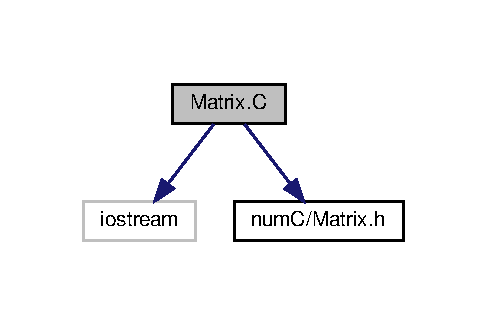
\includegraphics[width=234pt]{Matrix_8C__incl}
\end{center}
\end{figure}
\subsubsection*{Functions}
\begin{DoxyCompactItemize}
\item 
double $\ast$$\ast$ \hyperlink{Matrix_8C_a66ed07559a4d20174040e69f551a5431}{sum} (double $\ast$$\ast$mat1, double $\ast$$\ast$mat2, int a, int b)
\begin{DoxyCompactList}\small\item\em Elementwise summation. \end{DoxyCompactList}\item 
double $\ast$$\ast$ \hyperlink{Matrix_8C_a238af1517ec23a6f0279ec5ee6364d6a}{sub} (double $\ast$$\ast$mat1, double $\ast$$\ast$mat2, int a, int b)
\begin{DoxyCompactList}\small\item\em Elementwise subtraction. \end{DoxyCompactList}\item 
double $\ast$$\ast$ \hyperlink{Matrix_8C_a74a9fe9c1d326c41a69926c97720f4d2}{matmul} (double $\ast$$\ast$mat1, double $\ast$$\ast$mat2, int a, int b, int c)
\begin{DoxyCompactList}\small\item\em \hyperlink{classMatrix}{Matrix} multiplication. \end{DoxyCompactList}\item 
double $\ast$$\ast$ \hyperlink{Matrix_8C_ab64223fbcc37cc3af54071e71067d05a}{transpose} (double $\ast$$\ast$mat, int a, int b)
\begin{DoxyCompactList}\small\item\em \hyperlink{classMatrix}{Matrix} transpose. \end{DoxyCompactList}\item 
double $\ast$$\ast$ \hyperlink{Matrix_8C_affa4629470e427c236e2a7ac925e4e73}{identity} (int a, double val)
\begin{DoxyCompactList}\small\item\em Identity matrix. \end{DoxyCompactList}\item 
double $\ast$$\ast$ \hyperlink{Matrix_8C_a8f5f4f6401312604aebc715cca176985}{mat\+\_\+copy} (double $\ast$$\ast$mat, int a, int b)
\begin{DoxyCompactList}\small\item\em Hard copy matrix. \end{DoxyCompactList}\item 
double $\ast$$\ast$ \hyperlink{Matrix_8C_a19adaf60a005ffeb9071a395d0ee069f}{inverse} (double $\ast$$\ast$A, int a, int b)
\begin{DoxyCompactList}\small\item\em \hyperlink{classMatrix}{Matrix} left inverse. \end{DoxyCompactList}\item 
double $\ast$$\ast$ \hyperlink{Matrix_8C_ab8a4d647abae3e1b8dd318f1db696bc6}{zero} (int a, int b)
\begin{DoxyCompactList}\small\item\em Initialize matrix. \end{DoxyCompactList}\item 
void \hyperlink{Matrix_8C_a9c8e250ed43efa25186112ef66e4491f}{print} (double $\ast$$\ast$A, int a, int b)
\begin{DoxyCompactList}\small\item\em Print matrix. \end{DoxyCompactList}\end{DoxyCompactItemize}


\subsubsection{Detailed Description}
Various matrix operations. 

\begin{DoxyDate}{Date}
Mar 19, 2021 
\end{DoxyDate}
\begin{DoxyAuthor}{Author}
C J Park ~\newline
 \href{mailto:chanjure@snu.ac.kr}{\tt chanjure@snu.\+ac.\+kr} 
\end{DoxyAuthor}


\subsubsection{Function Documentation}
\mbox{\Hypertarget{Matrix_8C_affa4629470e427c236e2a7ac925e4e73}\label{Matrix_8C_affa4629470e427c236e2a7ac925e4e73}} 
\index{Matrix.\+C@{Matrix.\+C}!identity@{identity}}
\index{identity@{identity}!Matrix.\+C@{Matrix.\+C}}
\paragraph{\texorpdfstring{identity()}{identity()}}
{\footnotesize\ttfamily double$\ast$$\ast$ identity (\begin{DoxyParamCaption}\item[{int}]{,  }\item[{double}]{val = {\ttfamily 1.} }\end{DoxyParamCaption})}



Identity matrix. 

create identity matrix of given size square matrix will be created

Parameters\+: 
\begin{DoxyParams}{Parameters}
{\em a} & (int) dimension of identity matrix \\
\hline
{\em val} & (double) value to initalize (default = 1.)\\
\hline
\end{DoxyParams}
Returns\+: \begin{DoxyReturn}{Returns}
result (double$\ast$$\ast$) identity matrix
\end{DoxyReturn}
Example\+:

A = identity(3, 0.\+5);

Tag\+: identity initalize 

Definition at line 88 of file Matrix.\+C.



Referenced by inverse().


\begin{DoxyCode}
88                                     \{
89     \textcolor{keyword}{static} \textcolor{keywordtype}{double}** result;
90 
91     result = \textcolor{keyword}{new} \textcolor{keywordtype}{double}*[a];
92     \textcolor{keywordflow}{for}(\textcolor{keywordtype}{int} i=0;i<a;i++) *(result+i) = \textcolor{keyword}{new} \textcolor{keywordtype}{double} [a];
93 
94     \textcolor{keywordflow}{for}(\textcolor{keywordtype}{int} i=0;i<a;i++)\{
95         \textcolor{keywordflow}{for}(\textcolor{keywordtype}{int} j=0;j<a;j++)\{
96             \textcolor{keywordflow}{if}(i==j) *(*(result+i)+j) = val;
97             \textcolor{keywordflow}{else} *(*(result+i)+j) = 0.;
98         \}
99     \}
100 
101     \textcolor{keywordflow}{return} result;
102 \}
\end{DoxyCode}
\mbox{\Hypertarget{Matrix_8C_a19adaf60a005ffeb9071a395d0ee069f}\label{Matrix_8C_a19adaf60a005ffeb9071a395d0ee069f}} 
\index{Matrix.\+C@{Matrix.\+C}!inverse@{inverse}}
\index{inverse@{inverse}!Matrix.\+C@{Matrix.\+C}}
\paragraph{\texorpdfstring{inverse()}{inverse()}}
{\footnotesize\ttfamily double$\ast$$\ast$ inverse (\begin{DoxyParamCaption}\item[{double $\ast$$\ast$}]{,  }\item[{int}]{,  }\item[{int}]{ }\end{DoxyParamCaption})}



\hyperlink{classMatrix}{Matrix} left inverse. 

\hyperlink{classMatrix}{Matrix} left inverse using Gaussian reduction

Parameters\+: 
\begin{DoxyParams}{Parameters}
{\em A} & (double$\ast$$\ast$) matrix to inverse \\
\hline
{\em a} & (int) number of rows of A \\
\hline
{\em b} & (int) number of columns of A\\
\hline
\end{DoxyParams}
Returns\+: \begin{DoxyReturn}{Returns}
result (double$\ast$$\ast$) left inverse of A
\end{DoxyReturn}
Example\+:

A\+\_\+inv = inverse(\+A,2,2);

Tag\+: left inverse gaussian reduction 

Definition at line 117 of file Matrix.\+C.



References identity(), mat\+\_\+copy(), matmul(), print(), and transpose().


\begin{DoxyCode}
117                                           \{
118 
119     \textcolor{keyword}{static} \textcolor{keywordtype}{double}** result; \textcolor{comment}{// output matmul(invsqA, A.T)}
120     \textcolor{keywordtype}{double}** sqA; \textcolor{comment}{// squarized matrix = matmul(A.transpose, A)}
121     \textcolor{keywordtype}{double}** invsqA; \textcolor{comment}{// inverse of squared A}
122     \textcolor{keywordtype}{double}** A\_t; \textcolor{comment}{// Transposed matrix}
123     \textcolor{keywordtype}{double}* row; \textcolor{comment}{// Temporary row container}
124     \textcolor{keywordtype}{double}* invrow; \textcolor{comment}{// Temporary row container for inverse matrix - memorize sort order}
125     \textcolor{keywordtype}{double} det; \textcolor{comment}{// determinant}
126     \textcolor{keywordtype}{double} pivot;
127 
128     \textcolor{keyword}{const} \textcolor{keywordtype}{double} tol = 1e-14;
129 
130     result = \textcolor{keyword}{new} \textcolor{keywordtype}{double}*[b];
131     \textcolor{keywordflow}{for}(\textcolor{keywordtype}{int} i=0;i<b;i++) *(result+i) = \textcolor{keyword}{new} \textcolor{keywordtype}{double} [a];
132 
133     sqA = \textcolor{keyword}{new} \textcolor{keywordtype}{double}*[b];
134     \textcolor{keywordflow}{for}(\textcolor{keywordtype}{int} i=0;i<b;i++) *(sqA+i) = \textcolor{keyword}{new} \textcolor{keywordtype}{double} [b];
135 
136     invsqA = \textcolor{keyword}{new} \textcolor{keywordtype}{double}*[b];
137     \textcolor{keywordflow}{for}(\textcolor{keywordtype}{int} i=0;i<b;i++) *(invsqA+i) = \textcolor{keyword}{new} \textcolor{keywordtype}{double} [b];
138 
139     row = \textcolor{keyword}{new} \textcolor{keywordtype}{double} [b];
140 
141     \textcolor{comment}{// Initially identity matrix for inverse matrix container.}
142     invsqA = \hyperlink{Matrix_8C_affa4629470e427c236e2a7ac925e4e73}{identity}(b); 
143         
144     \textcolor{comment}{// Initialize transposed matrix.}
145     A\_t = \textcolor{keyword}{new} \textcolor{keywordtype}{double}*[b];
146     \textcolor{keywordflow}{for}(\textcolor{keywordtype}{int} i=0; i<b;i++) *(A\_t+i) = \textcolor{keyword}{new} \textcolor{keywordtype}{double} [b];
147     
148     \textcolor{keywordflow}{if}(a!=b)\{    
149         A\_t = \hyperlink{Matrix_8C_ab64223fbcc37cc3af54071e71067d05a}{transpose}(A,a,b);
150         \textcolor{comment}{// Squarize the matrix}
151         \textcolor{keywordflow}{for}(\textcolor{keywordtype}{int} i=0;i<b;i++)\{
152             \textcolor{keywordflow}{for}(\textcolor{keywordtype}{int} j=0;j<b;j++)\{
153                 \textcolor{keywordflow}{for}(\textcolor{keywordtype}{int} k=0;k<a;k++)\{
154                     *(*(sqA+i)+j) = *(*(A\_t+i)+k) * *(*(A+k)+j);
155                 \}
156             \}
157         \}
158     \}
159     \textcolor{keywordflow}{else}\{
160         A\_t = \hyperlink{Matrix_8C_affa4629470e427c236e2a7ac925e4e73}{identity}(a);
161         sqA = \hyperlink{Matrix_8C_a8f5f4f6401312604aebc715cca176985}{mat\_copy}(A,a,a);
162     \}
163 
164     \textcolor{comment}{// Sort pivot}
165     \textcolor{keywordflow}{for}(\textcolor{keywordtype}{int} j=0;j<b;j++)\{
166         \textcolor{keywordtype}{int} i = 1;
167         \textcolor{keywordflow}{while}(*(*(sqA+j)+j) <=tol && i<b)\{
168             \textcolor{comment}{// Save zero pivot row}
169             row = *(sqA+j);
170             invrow = *(invsqA+j);
171             
172             \textcolor{comment}{// Exchange with row below}
173             *(sqA+j) = *(sqA+j+i);
174             *(invsqA+j) = *(invsqA+j+i);
175 
176             *(sqA+j+i) = row;
177             *(invsqA+j+i) = invrow;
178 
179             i++;
180         \}
181     \}
182     \hyperlink{Matrix_8C_a9c8e250ed43efa25186112ef66e4491f}{print}(sqA,3,3);
183 
184     \textcolor{comment}{// Gauss Jordan method}
185     \textcolor{keywordflow}{for}(\textcolor{keywordtype}{int} i=0;i<b;i++)\{
186         \textcolor{comment}{// Scale}
187         pivot = *(*(sqA+i)+i);
188         printf(\textcolor{stringliteral}{"pivot : %f\(\backslash\)n"},pivot);
189         \textcolor{keywordflow}{if}(pivot!=1.)\{
190             \textcolor{keywordflow}{for}(\textcolor{keywordtype}{int} j=0;j<b;j++)\{
191                 *(*(invsqA+i)+j)/=pivot;
192                 *(*(sqA+i)+j)/=pivot;
193             \}
194         \}
195         \textcolor{comment}{// Subtraction}
196         \textcolor{keywordflow}{for}(\textcolor{keywordtype}{int} j=0;j<b;j++)\{
197             \textcolor{keywordflow}{if}(j!=i)\{
198                 \textcolor{keywordtype}{double} target = *(*(sqA+j)+i);
199                 \textcolor{keywordflow}{for}(\textcolor{keywordtype}{int} k=0;k<b;k++)\{
200                     *(*(invsqA+j)+k) -= *(*(invsqA+i)+k) * target;
201                     *(*(sqA+j)+k) -= *(*(sqA+i)+k) * target;
202                 \}
203             \}
204         \}
205     \}
206 
207     result = \hyperlink{Matrix_8C_a74a9fe9c1d326c41a69926c97720f4d2}{matmul}(invsqA, A\_t, b,b,a);
208 
209     \textcolor{keywordflow}{return} result;
210 \}
\end{DoxyCode}
\mbox{\Hypertarget{Matrix_8C_a8f5f4f6401312604aebc715cca176985}\label{Matrix_8C_a8f5f4f6401312604aebc715cca176985}} 
\index{Matrix.\+C@{Matrix.\+C}!mat\+\_\+copy@{mat\+\_\+copy}}
\index{mat\+\_\+copy@{mat\+\_\+copy}!Matrix.\+C@{Matrix.\+C}}
\paragraph{\texorpdfstring{mat\+\_\+copy()}{mat\_copy()}}
{\footnotesize\ttfamily double$\ast$$\ast$ mat\+\_\+copy (\begin{DoxyParamCaption}\item[{double $\ast$$\ast$}]{,  }\item[{int}]{,  }\item[{int}]{ }\end{DoxyParamCaption})}



Hard copy matrix. 

create hard copy of given matrix

Parameters\+: 
\begin{DoxyParams}{Parameters}
{\em mat} & (double$\ast$$\ast$) matrix to copy \\
\hline
{\em a} & (int) number of rows of mat \\
\hline
{\em b} & (int) number of columns of mat\\
\hline
\end{DoxyParams}
Returns\+: \begin{DoxyReturn}{Returns}
result (double$\ast$$\ast$) hard copy of mat
\end{DoxyReturn}
Example\+:

A = mat\+\_\+copy(\+B,3,3);

Tag\+: ftn 

Definition at line 104 of file Matrix.\+C.



Referenced by inverse().


\begin{DoxyCode}
104                                              \{
105     \textcolor{keyword}{static} \textcolor{keywordtype}{double}** result;
106 
107     result = \textcolor{keyword}{new} \textcolor{keywordtype}{double}*[a];
108     \textcolor{keywordflow}{for}(\textcolor{keywordtype}{int} i=0;i<a;i++) *(result+i) = \textcolor{keyword}{new} \textcolor{keywordtype}{double} [b];
109 
110     \textcolor{keywordflow}{for}(\textcolor{keywordtype}{int} i=0;i<a;i++)\{
111         \textcolor{keywordflow}{for}(\textcolor{keywordtype}{int} j=0;j<b;j++) *(*(result+i)+j) = *(*(mat+i)+j);
112     \}
113 
114     \textcolor{keywordflow}{return} result;
115 \}
\end{DoxyCode}
\mbox{\Hypertarget{Matrix_8C_a74a9fe9c1d326c41a69926c97720f4d2}\label{Matrix_8C_a74a9fe9c1d326c41a69926c97720f4d2}} 
\index{Matrix.\+C@{Matrix.\+C}!matmul@{matmul}}
\index{matmul@{matmul}!Matrix.\+C@{Matrix.\+C}}
\paragraph{\texorpdfstring{matmul()}{matmul()}}
{\footnotesize\ttfamily double$\ast$$\ast$ matmul (\begin{DoxyParamCaption}\item[{double $\ast$$\ast$}]{,  }\item[{double $\ast$$\ast$}]{,  }\item[{int}]{,  }\item[{int}]{,  }\item[{int}]{ }\end{DoxyParamCaption})}



\hyperlink{classMatrix}{Matrix} multiplication. 

mat1 $\ast$ mat2 = result number of column of mat1 must match number of column of mat2

Parameters\+: 
\begin{DoxyParams}{Parameters}
{\em mat1,mat2} & (double$\ast$$\ast$) matrices to be multiplied \\
\hline
{\em a} & (int) number of rows of mat1 \\
\hline
{\em b} & (int) number of folumns of mat1 = number of rows of mat2 \\
\hline
{\em c} & (int) number of columns of mat2\\
\hline
\end{DoxyParams}
Returns\+: \begin{DoxyReturn}{Returns}
result (double$\ast$$\ast$) matrix of dimension a x c
\end{DoxyReturn}
Example\+:

A = matmul(\+A,\+B,2,3,2);

Tag\+: multiplication 

Definition at line 45 of file Matrix.\+C.



Referenced by chisqr(), and inverse().


\begin{DoxyCode}
45                                                                   \{
46     
47     \textcolor{keyword}{static} \textcolor{keywordtype}{double}** result;
48     
49     result = \textcolor{keyword}{new} \textcolor{keywordtype}{double}*[a];
50     \textcolor{keywordflow}{for}(\textcolor{keywordtype}{int} i=0;i<a;i++) *(result + i) = \textcolor{keyword}{new} \textcolor{keywordtype}{double} [c];
51 
52     \textcolor{keywordflow}{for}(\textcolor{keywordtype}{int} i=0;i<a;i++)\{
53         \textcolor{keywordflow}{for}(\textcolor{keywordtype}{int} j=0;j<c;j++) *(*(result+i)+j) = 0.;
54     \}
55 
56     \textcolor{keywordflow}{for}(\textcolor{keywordtype}{int} i=0;i<a;i++)\{
57         \textcolor{keywordflow}{for}(\textcolor{keywordtype}{int} j=0;j<c;j++)\{
58             \textcolor{keywordflow}{for}(\textcolor{keywordtype}{int} k=0;k<b;k++)\{
59                 *(*(result+i)+j) += *(*(mat1+i)+k) * *(*(mat2+k)+j);
60             \}
61         \}
62     \}
63 
64     \textcolor{keywordflow}{return} result;
65 \}
\end{DoxyCode}
\mbox{\Hypertarget{Matrix_8C_a9c8e250ed43efa25186112ef66e4491f}\label{Matrix_8C_a9c8e250ed43efa25186112ef66e4491f}} 
\index{Matrix.\+C@{Matrix.\+C}!print@{print}}
\index{print@{print}!Matrix.\+C@{Matrix.\+C}}
\paragraph{\texorpdfstring{print()}{print()}}
{\footnotesize\ttfamily void print (\begin{DoxyParamCaption}\item[{double $\ast$$\ast$}]{,  }\item[{int}]{,  }\item[{int}]{ }\end{DoxyParamCaption})}



Print matrix. 

print matrix of given size

Parameters\+: 
\begin{DoxyParams}{Parameters}
{\em A} & (double$\ast$$\ast$) matrix to print \\
\hline
{\em a} & (int) number of rows of A \\
\hline
{\em b} & (int) number of columns of A\\
\hline
\end{DoxyParams}
Returns\+: \begin{DoxyReturn}{Returns}
stdout(matrix A)
\end{DoxyReturn}
Example\+:

print(\+A,2,3);

Tag\+: print 

Definition at line 225 of file Matrix.\+C.



Referenced by inverse().


\begin{DoxyCode}
225                                     \{
226     \textcolor{keywordflow}{for}(\textcolor{keywordtype}{int} i=0;i<a;i++)\{
227         \textcolor{keywordflow}{for}(\textcolor{keywordtype}{int} j=0;j<b;j++) printf(\textcolor{stringliteral}{"%10.4e "}, *(*(A+i)+j));
228         printf(\textcolor{stringliteral}{"\(\backslash\)n"});
229     \}
230 \}
\end{DoxyCode}
\mbox{\Hypertarget{Matrix_8C_a238af1517ec23a6f0279ec5ee6364d6a}\label{Matrix_8C_a238af1517ec23a6f0279ec5ee6364d6a}} 
\index{Matrix.\+C@{Matrix.\+C}!sub@{sub}}
\index{sub@{sub}!Matrix.\+C@{Matrix.\+C}}
\paragraph{\texorpdfstring{sub()}{sub()}}
{\footnotesize\ttfamily double$\ast$$\ast$ sub (\begin{DoxyParamCaption}\item[{double $\ast$$\ast$}]{,  }\item[{double $\ast$$\ast$}]{,  }\item[{int}]{,  }\item[{int}]{ }\end{DoxyParamCaption})}



Elementwise subtraction. 

mat1 -\/ mat2 = result Two input matrices must be in same shape axb

Parameters\+: 
\begin{DoxyParams}{Parameters}
{\em mat1,mat2} & (double$\ast$$\ast$) matrices to be subtracted \\
\hline
{\em a} & (int) number of rows of mat1 and mat2 \\
\hline
{\em b} & (int) number of columns of mat1 and mat2\\
\hline
\end{DoxyParams}
Returns\+: \begin{DoxyReturn}{Returns}
result (double$\ast$$\ast$)
\end{DoxyReturn}
Example\+:

A = sub(\+A,\+B,2,2);

Tag\+: subtract, element wise 

Definition at line 31 of file Matrix.\+C.



Referenced by chisqr().


\begin{DoxyCode}
31                                                         \{
32     
33     \textcolor{keyword}{static} \textcolor{keywordtype}{double}** result;
34 
35     result = \textcolor{keyword}{new} \textcolor{keywordtype}{double}*[a];
36     \textcolor{keywordflow}{for}(\textcolor{keywordtype}{int} i=0;i<a;i++) *(result+i) = \textcolor{keyword}{new} \textcolor{keywordtype}{double} [b];
37 
38     \textcolor{keywordflow}{for}(\textcolor{keywordtype}{int} i=0;i<a;i++)\{
39         \textcolor{keywordflow}{for}(\textcolor{keywordtype}{int} j=0;j<b;j++) *(*(result+i)+j) = *(*(mat1+i)+j) - *(*(mat2+i)+j);
40     \}
41 
42     \textcolor{keywordflow}{return} result;
43 \}
\end{DoxyCode}
\mbox{\Hypertarget{Matrix_8C_a66ed07559a4d20174040e69f551a5431}\label{Matrix_8C_a66ed07559a4d20174040e69f551a5431}} 
\index{Matrix.\+C@{Matrix.\+C}!sum@{sum}}
\index{sum@{sum}!Matrix.\+C@{Matrix.\+C}}
\paragraph{\texorpdfstring{sum()}{sum()}}
{\footnotesize\ttfamily double$\ast$$\ast$ sum (\begin{DoxyParamCaption}\item[{double $\ast$$\ast$}]{,  }\item[{double $\ast$$\ast$}]{,  }\item[{int}]{,  }\item[{int}]{ }\end{DoxyParamCaption})}



Elementwise summation. 

mat1 + mat2 = result Two input matrices must be in same shape axb

Parameters\+: 
\begin{DoxyParams}{Parameters}
{\em mat1,mat2} & (double$\ast$$\ast$) matrices to be added \\
\hline
{\em a} & (int) number of rows of mat1 and mat2 \\
\hline
{\em b} & (int) number of columns of mat1 and mat2\\
\hline
\end{DoxyParams}
Returns\+: \begin{DoxyReturn}{Returns}
result (double$\ast$$\ast$)
\end{DoxyReturn}
Example\+:

A = sum(\+A,\+B,2,2);

Tag\+: add, sum, element wise 

Definition at line 17 of file Matrix.\+C.


\begin{DoxyCode}
17                                                         \{
18     
19     \textcolor{keyword}{static} \textcolor{keywordtype}{double}** result;
20 
21     result = \textcolor{keyword}{new} \textcolor{keywordtype}{double}*[a];
22     \textcolor{keywordflow}{for}(\textcolor{keywordtype}{int} i=0;i<a;i++) *(result+i) = \textcolor{keyword}{new} \textcolor{keywordtype}{double} [b];
23 
24     \textcolor{keywordflow}{for}(\textcolor{keywordtype}{int} i=0;i<a;i++)\{
25         \textcolor{keywordflow}{for}(\textcolor{keywordtype}{int} j=0;j<b;j++) *(*(result+i)+j) = *(*(mat1+i)+j) + *(*(mat2+i)+j);
26     \}
27 
28     \textcolor{keywordflow}{return} result;
29 \}
\end{DoxyCode}
\mbox{\Hypertarget{Matrix_8C_ab64223fbcc37cc3af54071e71067d05a}\label{Matrix_8C_ab64223fbcc37cc3af54071e71067d05a}} 
\index{Matrix.\+C@{Matrix.\+C}!transpose@{transpose}}
\index{transpose@{transpose}!Matrix.\+C@{Matrix.\+C}}
\paragraph{\texorpdfstring{transpose()}{transpose()}}
{\footnotesize\ttfamily double$\ast$$\ast$ transpose (\begin{DoxyParamCaption}\item[{double $\ast$$\ast$}]{,  }\item[{int}]{,  }\item[{int}]{ }\end{DoxyParamCaption})}



\hyperlink{classMatrix}{Matrix} transpose. 

mat$^\wedge$T

Parameters\+: 
\begin{DoxyParams}{Parameters}
{\em mat} & (double$\ast$$\ast$) matrix to be transposed \\
\hline
{\em a} & (int) number of rows of mat \\
\hline
{\em b} & (int) number of columns of mat\\
\hline
\end{DoxyParams}
Returns\+: \begin{DoxyReturn}{Returns}
result (double$\ast$$\ast$) transposed mat
\end{DoxyReturn}
Example\+:

A\+\_\+T = transpose(\+A,2,2);

Tag\+: transpose 

Definition at line 67 of file Matrix.\+C.



Referenced by inverse().


\begin{DoxyCode}
67                                               \{
68 
69     \textcolor{keyword}{static} \textcolor{keywordtype}{double}** result;
70 
71     result = \textcolor{keyword}{new} \textcolor{keywordtype}{double}*[b];
72     \textcolor{keywordflow}{for}(\textcolor{keywordtype}{int} i=0;i<b;i++) *(result+i) = \textcolor{keyword}{new} \textcolor{keywordtype}{double} [a];
73 
74     \textcolor{keywordflow}{for}(\textcolor{keywordtype}{int} i=0;i<a;i++)\{
75         \textcolor{keywordflow}{for}(\textcolor{keywordtype}{int} j=0;j<b;j++)\{
76             *(*(result+j)+i) = *(*(mat+i)+j);
77         \}
78     \}
79 
80     \textcolor{keywordflow}{return} result;
81 \}
\end{DoxyCode}
\mbox{\Hypertarget{Matrix_8C_ab8a4d647abae3e1b8dd318f1db696bc6}\label{Matrix_8C_ab8a4d647abae3e1b8dd318f1db696bc6}} 
\index{Matrix.\+C@{Matrix.\+C}!zero@{zero}}
\index{zero@{zero}!Matrix.\+C@{Matrix.\+C}}
\paragraph{\texorpdfstring{zero()}{zero()}}
{\footnotesize\ttfamily double$\ast$$\ast$ zero (\begin{DoxyParamCaption}\item[{int}]{,  }\item[{int}]{ }\end{DoxyParamCaption})}



Initialize matrix. 

Create and initialize matrix elements to zero

Parameters\+: 
\begin{DoxyParams}{Parameters}
{\em a} & (int) number of rows \\
\hline
{\em b} & (int) number of columns\\
\hline
\end{DoxyParams}
Returns\+: \begin{DoxyReturn}{Returns}
result (double$\ast$$\ast$) zero matrix of size axb
\end{DoxyReturn}
Example\+:

A = zero(2,3);

Tag\+: initalize zero 

Definition at line 212 of file Matrix.\+C.


\begin{DoxyCode}
212                            \{
213     \textcolor{keyword}{static} \textcolor{keywordtype}{double}** result;
214     
215     result = \textcolor{keyword}{new} \textcolor{keywordtype}{double}*[a];
216     \textcolor{keywordflow}{for}(\textcolor{keywordtype}{int} i=0;i<a;i++) *(result+i) = \textcolor{keyword}{new} \textcolor{keywordtype}{double} [b];
217 
218     \textcolor{keywordflow}{for}(\textcolor{keywordtype}{int} i=0;i<a;i++)\{
219         \textcolor{keywordflow}{for}(\textcolor{keywordtype}{int} j=0;j<b;j++) *(*(result+i)+j) = 0.;
220     \}
221     
222     \textcolor{keywordflow}{return} result;
223 \}
\end{DoxyCode}

\hypertarget{Matrix_8h}{}\subsection{Matrix.\+h File Reference}
\label{Matrix_8h}\index{Matrix.\+h@{Matrix.\+h}}


Header file for \hyperlink{classMatrix}{Matrix} algebra.  


This graph shows which files directly or indirectly include this file\+:
\nopagebreak
\begin{figure}[H]
\begin{center}
\leavevmode
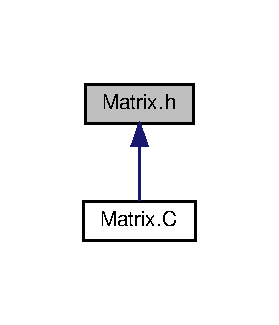
\includegraphics[width=134pt]{Matrix_8h__dep__incl}
\end{center}
\end{figure}
\subsubsection*{Functions}
\begin{DoxyCompactItemize}
\item 
double $\ast$$\ast$ \hyperlink{Matrix_8h_a21f00d2a3c50f395256c7800fefc6cf0}{sum} (double $\ast$$\ast$, double $\ast$$\ast$, int, int)
\begin{DoxyCompactList}\small\item\em Elementwise summation. \end{DoxyCompactList}\item 
double $\ast$$\ast$ \hyperlink{Matrix_8h_a173e1efd1a2864cfd7af0024b56915b4}{sub} (double $\ast$$\ast$, double $\ast$$\ast$, int, int)
\begin{DoxyCompactList}\small\item\em Elementwise subtraction. \end{DoxyCompactList}\item 
double $\ast$$\ast$ \hyperlink{Matrix_8h_a252d5999b5cca59570cf8f85567eef35}{matmul} (double $\ast$$\ast$, double $\ast$$\ast$, int, int, int)
\begin{DoxyCompactList}\small\item\em \hyperlink{classMatrix}{Matrix} multiplication. \end{DoxyCompactList}\item 
double $\ast$$\ast$ \hyperlink{Matrix_8h_add8d97520d6f45f114ee07b3b331c29d}{transpose} (double $\ast$$\ast$, int, int)
\begin{DoxyCompactList}\small\item\em \hyperlink{classMatrix}{Matrix} transpose. \end{DoxyCompactList}\item 
double $\ast$$\ast$ \hyperlink{Matrix_8h_ac0497c746531e3d9117e80b16cfe7b18}{inverse} (double $\ast$$\ast$, int, int)
\begin{DoxyCompactList}\small\item\em \hyperlink{classMatrix}{Matrix} left inverse. \end{DoxyCompactList}\item 
double $\ast$$\ast$ \hyperlink{Matrix_8h_a195dfe7c58ef9a9210e854a11a60e5d8}{identity} (int, double val=1.)
\begin{DoxyCompactList}\small\item\em Identity matrix. \end{DoxyCompactList}\item 
double $\ast$$\ast$ \hyperlink{Matrix_8h_abc83706f875424082d1710d14c5fe4d0}{mat\+\_\+copy} (double $\ast$$\ast$, int, int)
\begin{DoxyCompactList}\small\item\em Hard copy matrix. \end{DoxyCompactList}\item 
double $\ast$$\ast$ \hyperlink{Matrix_8h_aafe678a58e6896112ada70ec83a3f4af}{zero} (int, int)
\begin{DoxyCompactList}\small\item\em Initialize matrix. \end{DoxyCompactList}\item 
void \hyperlink{Matrix_8h_aa64d0eab19c69e019b28eda004b3a804}{print} (double $\ast$$\ast$, int, int)
\begin{DoxyCompactList}\small\item\em Print matrix. \end{DoxyCompactList}\end{DoxyCompactItemize}


\subsubsection{Detailed Description}
Header file for \hyperlink{classMatrix}{Matrix} algebra. 

\begin{DoxyDate}{Date}
Mar 19, 2021 
\end{DoxyDate}
\begin{DoxyAuthor}{Author}
C J Park ~\newline
 \href{mailto:chanjure@snu.ac.kr}{\tt chanjure@snu.\+ac.\+kr} 
\end{DoxyAuthor}
\begin{DoxyRefDesc}{Bug}
\item[\hyperlink{bug__bug000001}{Bug}]No known bugs. \end{DoxyRefDesc}
\begin{DoxyVersion}{Version}
0.\+1 
\end{DoxyVersion}


\subsubsection{Function Documentation}
\mbox{\Hypertarget{Matrix_8h_a195dfe7c58ef9a9210e854a11a60e5d8}\label{Matrix_8h_a195dfe7c58ef9a9210e854a11a60e5d8}} 
\index{Matrix.\+h@{Matrix.\+h}!identity@{identity}}
\index{identity@{identity}!Matrix.\+h@{Matrix.\+h}}
\paragraph{\texorpdfstring{identity()}{identity()}}
{\footnotesize\ttfamily double$\ast$$\ast$ identity (\begin{DoxyParamCaption}\item[{int}]{,  }\item[{double}]{val = {\ttfamily 1.} }\end{DoxyParamCaption})}



Identity matrix. 

create identity matrix of given size square matrix will be created

Parameters\+: 
\begin{DoxyParams}{Parameters}
{\em a} & (int) dimension of identity matrix \\
\hline
{\em val} & (double) value to initalize (default = 1.)\\
\hline
\end{DoxyParams}
Returns\+: \begin{DoxyReturn}{Returns}
result (double$\ast$$\ast$) identity matrix
\end{DoxyReturn}
Example\+:

A = identity(3, 0.\+5);

Tag\+: identity initalize 

Definition at line 88 of file Matrix.\+C.



Referenced by inverse().


\begin{DoxyCode}
88                                     \{
89     \textcolor{keyword}{static} \textcolor{keywordtype}{double}** result;
90 
91     result = \textcolor{keyword}{new} \textcolor{keywordtype}{double}*[a];
92     \textcolor{keywordflow}{for}(\textcolor{keywordtype}{int} i=0;i<a;i++) *(result+i) = \textcolor{keyword}{new} \textcolor{keywordtype}{double} [a];
93 
94     \textcolor{keywordflow}{for}(\textcolor{keywordtype}{int} i=0;i<a;i++)\{
95         \textcolor{keywordflow}{for}(\textcolor{keywordtype}{int} j=0;j<a;j++)\{
96             \textcolor{keywordflow}{if}(i==j) *(*(result+i)+j) = val;
97             \textcolor{keywordflow}{else} *(*(result+i)+j) = 0.;
98         \}
99     \}
100 
101     \textcolor{keywordflow}{return} result;
102 \}
\end{DoxyCode}
\mbox{\Hypertarget{Matrix_8h_ac0497c746531e3d9117e80b16cfe7b18}\label{Matrix_8h_ac0497c746531e3d9117e80b16cfe7b18}} 
\index{Matrix.\+h@{Matrix.\+h}!inverse@{inverse}}
\index{inverse@{inverse}!Matrix.\+h@{Matrix.\+h}}
\paragraph{\texorpdfstring{inverse()}{inverse()}}
{\footnotesize\ttfamily double$\ast$$\ast$ inverse (\begin{DoxyParamCaption}\item[{double $\ast$$\ast$}]{,  }\item[{int}]{,  }\item[{int}]{ }\end{DoxyParamCaption})}



\hyperlink{classMatrix}{Matrix} left inverse. 

\hyperlink{classMatrix}{Matrix} left inverse using Gaussian reduction

Parameters\+: 
\begin{DoxyParams}{Parameters}
{\em A} & (double$\ast$$\ast$) matrix to inverse \\
\hline
{\em a} & (int) number of rows of A \\
\hline
{\em b} & (int) number of columns of A\\
\hline
\end{DoxyParams}
Returns\+: \begin{DoxyReturn}{Returns}
result (double$\ast$$\ast$) left inverse of A
\end{DoxyReturn}
Example\+:

A\+\_\+inv = inverse(\+A,2,2);

Tag\+: left inverse gaussian reduction 

Definition at line 117 of file Matrix.\+C.



References identity(), mat\+\_\+copy(), matmul(), print(), and transpose().


\begin{DoxyCode}
117                                           \{
118 
119     \textcolor{keyword}{static} \textcolor{keywordtype}{double}** result; \textcolor{comment}{// output matmul(invsqA, A.T)}
120     \textcolor{keywordtype}{double}** sqA; \textcolor{comment}{// squarized matrix = matmul(A.transpose, A)}
121     \textcolor{keywordtype}{double}** invsqA; \textcolor{comment}{// inverse of squared A}
122     \textcolor{keywordtype}{double}** A\_t; \textcolor{comment}{// Transposed matrix}
123     \textcolor{keywordtype}{double}* row; \textcolor{comment}{// Temporary row container}
124     \textcolor{keywordtype}{double}* invrow; \textcolor{comment}{// Temporary row container for inverse matrix - memorize sort order}
125     \textcolor{keywordtype}{double} det; \textcolor{comment}{// determinant}
126     \textcolor{keywordtype}{double} pivot;
127 
128     \textcolor{keyword}{const} \textcolor{keywordtype}{double} tol = 1e-14;
129 
130     result = \textcolor{keyword}{new} \textcolor{keywordtype}{double}*[b];
131     \textcolor{keywordflow}{for}(\textcolor{keywordtype}{int} i=0;i<b;i++) *(result+i) = \textcolor{keyword}{new} \textcolor{keywordtype}{double} [a];
132 
133     sqA = \textcolor{keyword}{new} \textcolor{keywordtype}{double}*[b];
134     \textcolor{keywordflow}{for}(\textcolor{keywordtype}{int} i=0;i<b;i++) *(sqA+i) = \textcolor{keyword}{new} \textcolor{keywordtype}{double} [b];
135 
136     invsqA = \textcolor{keyword}{new} \textcolor{keywordtype}{double}*[b];
137     \textcolor{keywordflow}{for}(\textcolor{keywordtype}{int} i=0;i<b;i++) *(invsqA+i) = \textcolor{keyword}{new} \textcolor{keywordtype}{double} [b];
138 
139     row = \textcolor{keyword}{new} \textcolor{keywordtype}{double} [b];
140 
141     \textcolor{comment}{// Initially identity matrix for inverse matrix container.}
142     invsqA = \hyperlink{Matrix_8C_affa4629470e427c236e2a7ac925e4e73}{identity}(b); 
143         
144     \textcolor{comment}{// Initialize transposed matrix.}
145     A\_t = \textcolor{keyword}{new} \textcolor{keywordtype}{double}*[b];
146     \textcolor{keywordflow}{for}(\textcolor{keywordtype}{int} i=0; i<b;i++) *(A\_t+i) = \textcolor{keyword}{new} \textcolor{keywordtype}{double} [b];
147     
148     \textcolor{keywordflow}{if}(a!=b)\{    
149         A\_t = \hyperlink{Matrix_8C_ab64223fbcc37cc3af54071e71067d05a}{transpose}(A,a,b);
150         \textcolor{comment}{// Squarize the matrix}
151         \textcolor{keywordflow}{for}(\textcolor{keywordtype}{int} i=0;i<b;i++)\{
152             \textcolor{keywordflow}{for}(\textcolor{keywordtype}{int} j=0;j<b;j++)\{
153                 \textcolor{keywordflow}{for}(\textcolor{keywordtype}{int} k=0;k<a;k++)\{
154                     *(*(sqA+i)+j) = *(*(A\_t+i)+k) * *(*(A+k)+j);
155                 \}
156             \}
157         \}
158     \}
159     \textcolor{keywordflow}{else}\{
160         A\_t = \hyperlink{Matrix_8C_affa4629470e427c236e2a7ac925e4e73}{identity}(a);
161         sqA = \hyperlink{Matrix_8C_a8f5f4f6401312604aebc715cca176985}{mat\_copy}(A,a,a);
162     \}
163 
164     \textcolor{comment}{// Sort pivot}
165     \textcolor{keywordflow}{for}(\textcolor{keywordtype}{int} j=0;j<b;j++)\{
166         \textcolor{keywordtype}{int} i = 1;
167         \textcolor{keywordflow}{while}(*(*(sqA+j)+j) <=tol && i<b)\{
168             \textcolor{comment}{// Save zero pivot row}
169             row = *(sqA+j);
170             invrow = *(invsqA+j);
171             
172             \textcolor{comment}{// Exchange with row below}
173             *(sqA+j) = *(sqA+j+i);
174             *(invsqA+j) = *(invsqA+j+i);
175 
176             *(sqA+j+i) = row;
177             *(invsqA+j+i) = invrow;
178 
179             i++;
180         \}
181     \}
182     \hyperlink{Matrix_8C_a9c8e250ed43efa25186112ef66e4491f}{print}(sqA,3,3);
183 
184     \textcolor{comment}{// Gauss Jordan method}
185     \textcolor{keywordflow}{for}(\textcolor{keywordtype}{int} i=0;i<b;i++)\{
186         \textcolor{comment}{// Scale}
187         pivot = *(*(sqA+i)+i);
188         printf(\textcolor{stringliteral}{"pivot : %f\(\backslash\)n"},pivot);
189         \textcolor{keywordflow}{if}(pivot!=1.)\{
190             \textcolor{keywordflow}{for}(\textcolor{keywordtype}{int} j=0;j<b;j++)\{
191                 *(*(invsqA+i)+j)/=pivot;
192                 *(*(sqA+i)+j)/=pivot;
193             \}
194         \}
195         \textcolor{comment}{// Subtraction}
196         \textcolor{keywordflow}{for}(\textcolor{keywordtype}{int} j=0;j<b;j++)\{
197             \textcolor{keywordflow}{if}(j!=i)\{
198                 \textcolor{keywordtype}{double} target = *(*(sqA+j)+i);
199                 \textcolor{keywordflow}{for}(\textcolor{keywordtype}{int} k=0;k<b;k++)\{
200                     *(*(invsqA+j)+k) -= *(*(invsqA+i)+k) * target;
201                     *(*(sqA+j)+k) -= *(*(sqA+i)+k) * target;
202                 \}
203             \}
204         \}
205     \}
206 
207     result = \hyperlink{Matrix_8C_a74a9fe9c1d326c41a69926c97720f4d2}{matmul}(invsqA, A\_t, b,b,a);
208 
209     \textcolor{keywordflow}{return} result;
210 \}
\end{DoxyCode}
\mbox{\Hypertarget{Matrix_8h_abc83706f875424082d1710d14c5fe4d0}\label{Matrix_8h_abc83706f875424082d1710d14c5fe4d0}} 
\index{Matrix.\+h@{Matrix.\+h}!mat\+\_\+copy@{mat\+\_\+copy}}
\index{mat\+\_\+copy@{mat\+\_\+copy}!Matrix.\+h@{Matrix.\+h}}
\paragraph{\texorpdfstring{mat\+\_\+copy()}{mat\_copy()}}
{\footnotesize\ttfamily double$\ast$$\ast$ mat\+\_\+copy (\begin{DoxyParamCaption}\item[{double $\ast$$\ast$}]{,  }\item[{int}]{,  }\item[{int}]{ }\end{DoxyParamCaption})}



Hard copy matrix. 

create hard copy of given matrix

Parameters\+: 
\begin{DoxyParams}{Parameters}
{\em mat} & (double$\ast$$\ast$) matrix to copy \\
\hline
{\em a} & (int) number of rows of mat \\
\hline
{\em b} & (int) number of columns of mat\\
\hline
\end{DoxyParams}
Returns\+: \begin{DoxyReturn}{Returns}
result (double$\ast$$\ast$) hard copy of mat
\end{DoxyReturn}
Example\+:

A = mat\+\_\+copy(\+B,3,3);

Tag\+: ftn 

Definition at line 104 of file Matrix.\+C.



Referenced by inverse().


\begin{DoxyCode}
104                                              \{
105     \textcolor{keyword}{static} \textcolor{keywordtype}{double}** result;
106 
107     result = \textcolor{keyword}{new} \textcolor{keywordtype}{double}*[a];
108     \textcolor{keywordflow}{for}(\textcolor{keywordtype}{int} i=0;i<a;i++) *(result+i) = \textcolor{keyword}{new} \textcolor{keywordtype}{double} [b];
109 
110     \textcolor{keywordflow}{for}(\textcolor{keywordtype}{int} i=0;i<a;i++)\{
111         \textcolor{keywordflow}{for}(\textcolor{keywordtype}{int} j=0;j<b;j++) *(*(result+i)+j) = *(*(mat+i)+j);
112     \}
113 
114     \textcolor{keywordflow}{return} result;
115 \}
\end{DoxyCode}
\mbox{\Hypertarget{Matrix_8h_a252d5999b5cca59570cf8f85567eef35}\label{Matrix_8h_a252d5999b5cca59570cf8f85567eef35}} 
\index{Matrix.\+h@{Matrix.\+h}!matmul@{matmul}}
\index{matmul@{matmul}!Matrix.\+h@{Matrix.\+h}}
\paragraph{\texorpdfstring{matmul()}{matmul()}}
{\footnotesize\ttfamily double$\ast$$\ast$ matmul (\begin{DoxyParamCaption}\item[{double $\ast$$\ast$}]{,  }\item[{double $\ast$$\ast$}]{,  }\item[{int}]{,  }\item[{int}]{,  }\item[{int}]{ }\end{DoxyParamCaption})}



\hyperlink{classMatrix}{Matrix} multiplication. 

mat1 $\ast$ mat2 = result number of column of mat1 must match number of column of mat2

Parameters\+: 
\begin{DoxyParams}{Parameters}
{\em mat1,mat2} & (double$\ast$$\ast$) matrices to be multiplied \\
\hline
{\em a} & (int) number of rows of mat1 \\
\hline
{\em b} & (int) number of folumns of mat1 = number of rows of mat2 \\
\hline
{\em c} & (int) number of columns of mat2\\
\hline
\end{DoxyParams}
Returns\+: \begin{DoxyReturn}{Returns}
result (double$\ast$$\ast$) matrix of dimension a x c
\end{DoxyReturn}
Example\+:

A = matmul(\+A,\+B,2,3,2);

Tag\+: multiplication 

Definition at line 45 of file Matrix.\+C.



Referenced by inverse().


\begin{DoxyCode}
45                                                                   \{
46     
47     \textcolor{keyword}{static} \textcolor{keywordtype}{double}** result;
48     
49     result = \textcolor{keyword}{new} \textcolor{keywordtype}{double}*[a];
50     \textcolor{keywordflow}{for}(\textcolor{keywordtype}{int} i=0;i<a;i++) *(result + i) = \textcolor{keyword}{new} \textcolor{keywordtype}{double} [c];
51 
52     \textcolor{keywordflow}{for}(\textcolor{keywordtype}{int} i=0;i<a;i++)\{
53         \textcolor{keywordflow}{for}(\textcolor{keywordtype}{int} j=0;j<c;j++) *(*(result+i)+j) = 0.;
54     \}
55 
56     \textcolor{keywordflow}{for}(\textcolor{keywordtype}{int} i=0;i<a;i++)\{
57         \textcolor{keywordflow}{for}(\textcolor{keywordtype}{int} j=0;j<c;j++)\{
58             \textcolor{keywordflow}{for}(\textcolor{keywordtype}{int} k=0;k<b;k++)\{
59                 *(*(result+i)+j) += *(*(mat1+i)+k) * *(*(mat2+k)+j);
60             \}
61         \}
62     \}
63 
64     \textcolor{keywordflow}{return} result;
65 \}
\end{DoxyCode}
\mbox{\Hypertarget{Matrix_8h_aa64d0eab19c69e019b28eda004b3a804}\label{Matrix_8h_aa64d0eab19c69e019b28eda004b3a804}} 
\index{Matrix.\+h@{Matrix.\+h}!print@{print}}
\index{print@{print}!Matrix.\+h@{Matrix.\+h}}
\paragraph{\texorpdfstring{print()}{print()}}
{\footnotesize\ttfamily void print (\begin{DoxyParamCaption}\item[{double $\ast$$\ast$}]{,  }\item[{int}]{,  }\item[{int}]{ }\end{DoxyParamCaption})}



Print matrix. 

print matrix of given size

Parameters\+: 
\begin{DoxyParams}{Parameters}
{\em A} & (double$\ast$$\ast$) matrix to print \\
\hline
{\em a} & (int) number of rows of A \\
\hline
{\em b} & (int) number of columns of A\\
\hline
\end{DoxyParams}
Returns\+: \begin{DoxyReturn}{Returns}
stdout(matrix A)
\end{DoxyReturn}
Example\+:

print(\+A,2,3);

Tag\+: print 

Definition at line 225 of file Matrix.\+C.



Referenced by inverse().


\begin{DoxyCode}
225                                     \{
226     \textcolor{keywordflow}{for}(\textcolor{keywordtype}{int} i=0;i<a;i++)\{
227         \textcolor{keywordflow}{for}(\textcolor{keywordtype}{int} j=0;j<b;j++) printf(\textcolor{stringliteral}{"%10.4e "}, *(*(A+i)+j));
228         printf(\textcolor{stringliteral}{"\(\backslash\)n"});
229     \}
230 \}
\end{DoxyCode}
\mbox{\Hypertarget{Matrix_8h_a173e1efd1a2864cfd7af0024b56915b4}\label{Matrix_8h_a173e1efd1a2864cfd7af0024b56915b4}} 
\index{Matrix.\+h@{Matrix.\+h}!sub@{sub}}
\index{sub@{sub}!Matrix.\+h@{Matrix.\+h}}
\paragraph{\texorpdfstring{sub()}{sub()}}
{\footnotesize\ttfamily double$\ast$$\ast$ sub (\begin{DoxyParamCaption}\item[{double $\ast$$\ast$}]{,  }\item[{double $\ast$$\ast$}]{,  }\item[{int}]{,  }\item[{int}]{ }\end{DoxyParamCaption})}



Elementwise subtraction. 

mat1 -\/ mat2 = result Two input matrices must be in same shape axb

Parameters\+: 
\begin{DoxyParams}{Parameters}
{\em mat1,mat2} & (double$\ast$$\ast$) matrices to be subtracted \\
\hline
{\em a} & (int) number of rows of mat1 and mat2 \\
\hline
{\em b} & (int) number of columns of mat1 and mat2\\
\hline
\end{DoxyParams}
Returns\+: \begin{DoxyReturn}{Returns}
result (double$\ast$$\ast$)
\end{DoxyReturn}
Example\+:

A = sub(\+A,\+B,2,2);

Tag\+: subtract, element wise 

Definition at line 31 of file Matrix.\+C.


\begin{DoxyCode}
31                                                         \{
32     
33     \textcolor{keyword}{static} \textcolor{keywordtype}{double}** result;
34 
35     result = \textcolor{keyword}{new} \textcolor{keywordtype}{double}*[a];
36     \textcolor{keywordflow}{for}(\textcolor{keywordtype}{int} i=0;i<a;i++) *(result+i) = \textcolor{keyword}{new} \textcolor{keywordtype}{double} [b];
37 
38     \textcolor{keywordflow}{for}(\textcolor{keywordtype}{int} i=0;i<a;i++)\{
39         \textcolor{keywordflow}{for}(\textcolor{keywordtype}{int} j=0;j<b;j++) *(*(result+i)+j) = *(*(mat1+i)+j) - *(*(mat2+i)+j);
40     \}
41 
42     \textcolor{keywordflow}{return} result;
43 \}
\end{DoxyCode}
\mbox{\Hypertarget{Matrix_8h_a21f00d2a3c50f395256c7800fefc6cf0}\label{Matrix_8h_a21f00d2a3c50f395256c7800fefc6cf0}} 
\index{Matrix.\+h@{Matrix.\+h}!sum@{sum}}
\index{sum@{sum}!Matrix.\+h@{Matrix.\+h}}
\paragraph{\texorpdfstring{sum()}{sum()}}
{\footnotesize\ttfamily double$\ast$$\ast$ sum (\begin{DoxyParamCaption}\item[{double $\ast$$\ast$}]{,  }\item[{double $\ast$$\ast$}]{,  }\item[{int}]{,  }\item[{int}]{ }\end{DoxyParamCaption})}



Elementwise summation. 

mat1 + mat2 = result Two input matrices must be in same shape axb

Parameters\+: 
\begin{DoxyParams}{Parameters}
{\em mat1,mat2} & (double$\ast$$\ast$) matrices to be added \\
\hline
{\em a} & (int) number of rows of mat1 and mat2 \\
\hline
{\em b} & (int) number of columns of mat1 and mat2\\
\hline
\end{DoxyParams}
Returns\+: \begin{DoxyReturn}{Returns}
result (double$\ast$$\ast$)
\end{DoxyReturn}
Example\+:

A = sum(\+A,\+B,2,2);

Tag\+: add, sum, element wise 

Definition at line 17 of file Matrix.\+C.


\begin{DoxyCode}
17                                                         \{
18     
19     \textcolor{keyword}{static} \textcolor{keywordtype}{double}** result;
20 
21     result = \textcolor{keyword}{new} \textcolor{keywordtype}{double}*[a];
22     \textcolor{keywordflow}{for}(\textcolor{keywordtype}{int} i=0;i<a;i++) *(result+i) = \textcolor{keyword}{new} \textcolor{keywordtype}{double} [b];
23 
24     \textcolor{keywordflow}{for}(\textcolor{keywordtype}{int} i=0;i<a;i++)\{
25         \textcolor{keywordflow}{for}(\textcolor{keywordtype}{int} j=0;j<b;j++) *(*(result+i)+j) = *(*(mat1+i)+j) + *(*(mat2+i)+j);
26     \}
27 
28     \textcolor{keywordflow}{return} result;
29 \}
\end{DoxyCode}
\mbox{\Hypertarget{Matrix_8h_add8d97520d6f45f114ee07b3b331c29d}\label{Matrix_8h_add8d97520d6f45f114ee07b3b331c29d}} 
\index{Matrix.\+h@{Matrix.\+h}!transpose@{transpose}}
\index{transpose@{transpose}!Matrix.\+h@{Matrix.\+h}}
\paragraph{\texorpdfstring{transpose()}{transpose()}}
{\footnotesize\ttfamily double$\ast$$\ast$ transpose (\begin{DoxyParamCaption}\item[{double $\ast$$\ast$}]{,  }\item[{int}]{,  }\item[{int}]{ }\end{DoxyParamCaption})}



\hyperlink{classMatrix}{Matrix} transpose. 

mat$^\wedge$T

Parameters\+: 
\begin{DoxyParams}{Parameters}
{\em mat} & (double$\ast$$\ast$) matrix to be transposed \\
\hline
{\em a} & (int) number of rows of mat \\
\hline
{\em b} & (int) number of columns of mat\\
\hline
\end{DoxyParams}
Returns\+: \begin{DoxyReturn}{Returns}
result (double$\ast$$\ast$) transposed mat
\end{DoxyReturn}
Example\+:

A\+\_\+T = transpose(\+A,2,2);

Tag\+: transpose 

Definition at line 67 of file Matrix.\+C.



Referenced by inverse().


\begin{DoxyCode}
67                                               \{
68 
69     \textcolor{keyword}{static} \textcolor{keywordtype}{double}** result;
70 
71     result = \textcolor{keyword}{new} \textcolor{keywordtype}{double}*[b];
72     \textcolor{keywordflow}{for}(\textcolor{keywordtype}{int} i=0;i<b;i++) *(result+i) = \textcolor{keyword}{new} \textcolor{keywordtype}{double} [a];
73 
74     \textcolor{keywordflow}{for}(\textcolor{keywordtype}{int} i=0;i<a;i++)\{
75         \textcolor{keywordflow}{for}(\textcolor{keywordtype}{int} j=0;j<b;j++)\{
76             *(*(result+j)+i) = *(*(mat+i)+j);
77         \}
78     \}
79 
80     \textcolor{keywordflow}{return} result;
81 \}
\end{DoxyCode}
\mbox{\Hypertarget{Matrix_8h_aafe678a58e6896112ada70ec83a3f4af}\label{Matrix_8h_aafe678a58e6896112ada70ec83a3f4af}} 
\index{Matrix.\+h@{Matrix.\+h}!zero@{zero}}
\index{zero@{zero}!Matrix.\+h@{Matrix.\+h}}
\paragraph{\texorpdfstring{zero()}{zero()}}
{\footnotesize\ttfamily double$\ast$$\ast$ zero (\begin{DoxyParamCaption}\item[{int}]{,  }\item[{int}]{ }\end{DoxyParamCaption})}



Initialize matrix. 

Create and initialize matrix elements to zero

Parameters\+: 
\begin{DoxyParams}{Parameters}
{\em a} & (int) number of rows \\
\hline
{\em b} & (int) number of columns\\
\hline
\end{DoxyParams}
Returns\+: \begin{DoxyReturn}{Returns}
result (double$\ast$$\ast$) zero matrix of size axb
\end{DoxyReturn}
Example\+:

A = zero(2,3);

Tag\+: initalize zero 

Definition at line 212 of file Matrix.\+C.


\begin{DoxyCode}
212                            \{
213     \textcolor{keyword}{static} \textcolor{keywordtype}{double}** result;
214     
215     result = \textcolor{keyword}{new} \textcolor{keywordtype}{double}*[a];
216     \textcolor{keywordflow}{for}(\textcolor{keywordtype}{int} i=0;i<a;i++) *(result+i) = \textcolor{keyword}{new} \textcolor{keywordtype}{double} [b];
217 
218     \textcolor{keywordflow}{for}(\textcolor{keywordtype}{int} i=0;i<a;i++)\{
219         \textcolor{keywordflow}{for}(\textcolor{keywordtype}{int} j=0;j<b;j++) *(*(result+i)+j) = 0.;
220     \}
221     
222     \textcolor{keywordflow}{return} result;
223 \}
\end{DoxyCode}

\hypertarget{Matrix__gsl_8C}{}\subsection{Matrix\+\_\+gsl.\+C File Reference}
\label{Matrix__gsl_8C}\index{Matrix\+\_\+gsl.\+C@{Matrix\+\_\+gsl.\+C}}


\hyperlink{classMatrix}{Matrix} class functions using gsl library partially compatible with \hyperlink{Matrix_8h}{Matrix.\+h}.  


{\ttfamily \#include $<$gsl/gsl\+\_\+vector.\+h$>$}\newline
{\ttfamily \#include $<$gsl/gsl\+\_\+matrix.\+h$>$}\newline
{\ttfamily \#include $<$gsl/gsl\+\_\+linalg.\+h$>$}\newline
{\ttfamily \#include $<$num\+C/\+Matrix\+\_\+gsl.\+h$>$}\newline
Include dependency graph for Matrix\+\_\+gsl.\+C\+:\nopagebreak
\begin{figure}[H]
\begin{center}
\leavevmode
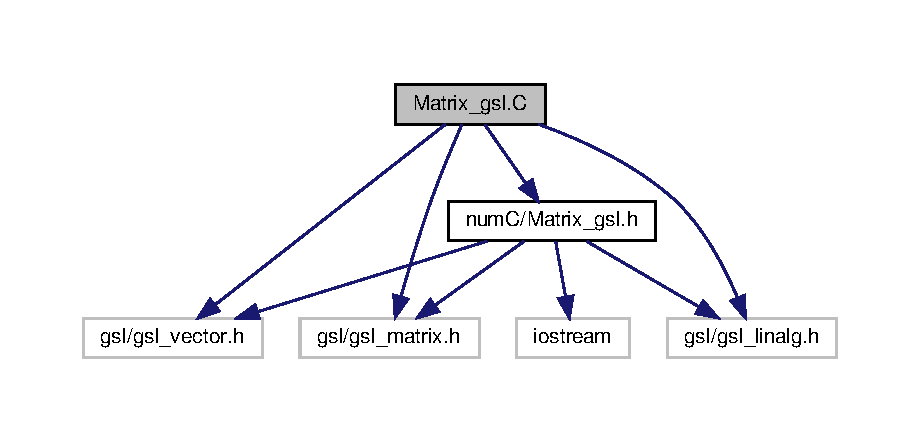
\includegraphics[width=350pt]{Matrix__gsl_8C__incl}
\end{center}
\end{figure}
\subsubsection*{Functions}
\begin{DoxyCompactItemize}
\item 
\mbox{\Hypertarget{Matrix__gsl_8C_a9300897ae0d96a9c6e599b5d054d467c}\label{Matrix__gsl_8C_a9300897ae0d96a9c6e599b5d054d467c}} 
\hyperlink{classMatrix}{Matrix} {\bfseries add} (\hyperlink{classMatrix}{Matrix} A, \hyperlink{classMatrix}{Matrix} B)
\item 
\mbox{\Hypertarget{Matrix__gsl_8C_afdb38b4e9def92cb3ba67e4895fdcb22}\label{Matrix__gsl_8C_afdb38b4e9def92cb3ba67e4895fdcb22}} 
\hyperlink{classMatrix}{Matrix} {\bfseries sub} (\hyperlink{classMatrix}{Matrix} A, \hyperlink{classMatrix}{Matrix} B)
\item 
\mbox{\Hypertarget{Matrix__gsl_8C_ac8e81b9762dbd22fb97ba543b9f7a3a8}\label{Matrix__gsl_8C_ac8e81b9762dbd22fb97ba543b9f7a3a8}} 
\hyperlink{classMatrix}{Matrix} {\bfseries mul} (\hyperlink{classMatrix}{Matrix} A, \hyperlink{classMatrix}{Matrix} B)
\item 
\mbox{\Hypertarget{Matrix__gsl_8C_ad89a5d42047fb5f90e6b16ba8e3c1717}\label{Matrix__gsl_8C_ad89a5d42047fb5f90e6b16ba8e3c1717}} 
\hyperlink{classMatrix}{Matrix} {\bfseries div} (\hyperlink{classMatrix}{Matrix} A, \hyperlink{classMatrix}{Matrix} B)
\item 
\mbox{\Hypertarget{Matrix__gsl_8C_aae80f28cb8803956de0c56c1618a7459}\label{Matrix__gsl_8C_aae80f28cb8803956de0c56c1618a7459}} 
\hyperlink{classMatrix}{Matrix} {\bfseries matmul} (\hyperlink{classMatrix}{Matrix} A, \hyperlink{classMatrix}{Matrix} B)
\item 
\mbox{\Hypertarget{Matrix__gsl_8C_a6b6043237c9821d9889356dc6ec120b7}\label{Matrix__gsl_8C_a6b6043237c9821d9889356dc6ec120b7}} 
\hyperlink{classMatrix}{Matrix} {\bfseries c\+\_\+} (\hyperlink{classMatrix}{Matrix} A, \hyperlink{classMatrix}{Matrix} B)
\item 
\mbox{\Hypertarget{Matrix__gsl_8C_a4cf258bad2d4532e818c44d52af46078}\label{Matrix__gsl_8C_a4cf258bad2d4532e818c44d52af46078}} 
\hyperlink{classMatrix}{Matrix} {\bfseries r\+\_\+} (\hyperlink{classMatrix}{Matrix} A, \hyperlink{classMatrix}{Matrix} B)
\item 
\mbox{\Hypertarget{Matrix__gsl_8C_ad150dfc63c53d24d88b344780c1f622f}\label{Matrix__gsl_8C_ad150dfc63c53d24d88b344780c1f622f}} 
double {\bfseries max} (double $\ast$$\ast$A, int n, int m)
\item 
\mbox{\Hypertarget{Matrix__gsl_8C_ab9bafe12f66bfe8e15fd56efa85ae061}\label{Matrix__gsl_8C_ab9bafe12f66bfe8e15fd56efa85ae061}} 
double {\bfseries min} (double $\ast$$\ast$A, int n, int m)
\end{DoxyCompactItemize}


\subsubsection{Detailed Description}
\hyperlink{classMatrix}{Matrix} class functions using gsl library partially compatible with \hyperlink{Matrix_8h}{Matrix.\+h}. 

Tag Index Imp \+: Could be improved 
\hypertarget{Matrix__gsl_8h}{}\subsection{Matrix\+\_\+gsl.\+h File Reference}
\label{Matrix__gsl_8h}\index{Matrix\+\_\+gsl.\+h@{Matrix\+\_\+gsl.\+h}}


\hyperlink{classMatrix}{Matrix} class and functions using gsl library.  


{\ttfamily \#include $<$iostream$>$}\newline
{\ttfamily \#include $<$gsl/gsl\+\_\+matrix.\+h$>$}\newline
{\ttfamily \#include $<$gsl/gsl\+\_\+vector.\+h$>$}\newline
{\ttfamily \#include $<$gsl/gsl\+\_\+linalg.\+h$>$}\newline
Include dependency graph for Matrix\+\_\+gsl.\+h\+:\nopagebreak
\begin{figure}[H]
\begin{center}
\leavevmode
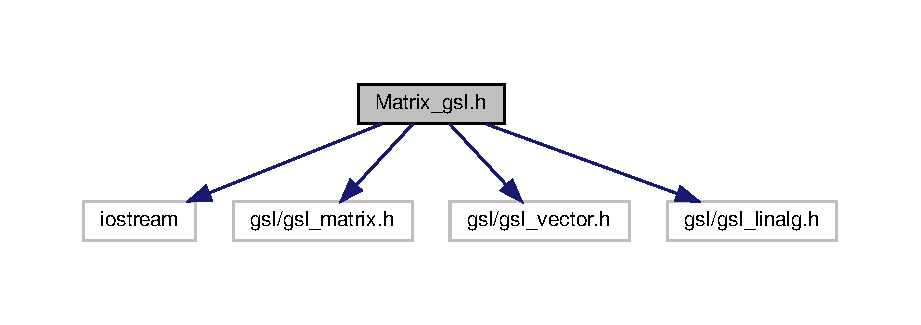
\includegraphics[width=350pt]{Matrix__gsl_8h__incl}
\end{center}
\end{figure}
This graph shows which files directly or indirectly include this file\+:\nopagebreak
\begin{figure}[H]
\begin{center}
\leavevmode
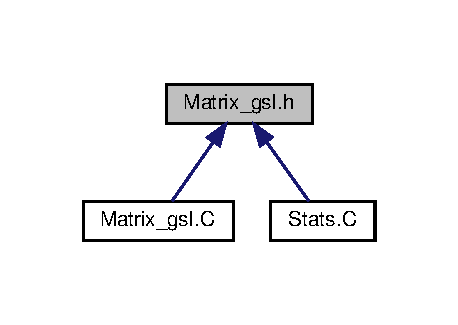
\includegraphics[width=220pt]{Matrix__gsl_8h__dep__incl}
\end{center}
\end{figure}
\subsubsection*{Data Structures}
\begin{DoxyCompactItemize}
\item 
class \hyperlink{classMatrix}{Matrix}
\begin{DoxyCompactList}\small\item\em This is \hyperlink{classMatrix}{Matrix} class. \end{DoxyCompactList}\end{DoxyCompactItemize}
\subsubsection*{Functions}
\begin{DoxyCompactItemize}
\item 
\mbox{\Hypertarget{Matrix__gsl_8h_ab588c2268c4490c4b2e0ae559858d09e}\label{Matrix__gsl_8h_ab588c2268c4490c4b2e0ae559858d09e}} 
\hyperlink{classMatrix}{Matrix} {\bfseries operator$\ast$} (\hyperlink{classMatrix}{Matrix} A, double a)
\item 
\mbox{\Hypertarget{Matrix__gsl_8h_aee5655304b39b1b087b45cb7af60631a}\label{Matrix__gsl_8h_aee5655304b39b1b087b45cb7af60631a}} 
\hyperlink{classMatrix}{Matrix} {\bfseries operator$\ast$} (double a, \hyperlink{classMatrix}{Matrix} A)
\item 
\mbox{\Hypertarget{Matrix__gsl_8h_a27778f7cde8a6fc394afd81fffaa0f8e}\label{Matrix__gsl_8h_a27778f7cde8a6fc394afd81fffaa0f8e}} 
\hyperlink{classMatrix}{Matrix} {\bfseries operator/} (\hyperlink{classMatrix}{Matrix} A, double a)
\item 
\mbox{\Hypertarget{Matrix__gsl_8h_ae46cddd1bbc69dbb102f0268082c7fcd}\label{Matrix__gsl_8h_ae46cddd1bbc69dbb102f0268082c7fcd}} 
\hyperlink{classMatrix}{Matrix} {\bfseries operator/} (double a, \hyperlink{classMatrix}{Matrix} A)
\item 
\mbox{\Hypertarget{Matrix__gsl_8h_a6727dbe57c0ffaada245b8a4d68a759f}\label{Matrix__gsl_8h_a6727dbe57c0ffaada245b8a4d68a759f}} 
\hyperlink{classMatrix}{Matrix} {\bfseries add} (\hyperlink{classMatrix}{Matrix}, \hyperlink{classMatrix}{Matrix})
\item 
\mbox{\Hypertarget{Matrix__gsl_8h_afb78d56f15a9b1705cef1c8321041554}\label{Matrix__gsl_8h_afb78d56f15a9b1705cef1c8321041554}} 
\hyperlink{classMatrix}{Matrix} {\bfseries sub} (\hyperlink{classMatrix}{Matrix}, \hyperlink{classMatrix}{Matrix})
\item 
\mbox{\Hypertarget{Matrix__gsl_8h_a78a111df182ae0cf09268fe8453802fe}\label{Matrix__gsl_8h_a78a111df182ae0cf09268fe8453802fe}} 
\hyperlink{classMatrix}{Matrix} {\bfseries mul} (\hyperlink{classMatrix}{Matrix}, \hyperlink{classMatrix}{Matrix})
\item 
\mbox{\Hypertarget{Matrix__gsl_8h_aeb8ab836584144d2fd99fab360c0ee7e}\label{Matrix__gsl_8h_aeb8ab836584144d2fd99fab360c0ee7e}} 
\hyperlink{classMatrix}{Matrix} {\bfseries div} (\hyperlink{classMatrix}{Matrix}, \hyperlink{classMatrix}{Matrix})
\item 
\mbox{\Hypertarget{Matrix__gsl_8h_a48c0fe9b6145483ff681527957a58787}\label{Matrix__gsl_8h_a48c0fe9b6145483ff681527957a58787}} 
\hyperlink{classMatrix}{Matrix} {\bfseries matmul} (\hyperlink{classMatrix}{Matrix}, \hyperlink{classMatrix}{Matrix})
\item 
\mbox{\Hypertarget{Matrix__gsl_8h_a81803854a9b64d7b7ffece43979806df}\label{Matrix__gsl_8h_a81803854a9b64d7b7ffece43979806df}} 
\hyperlink{classMatrix}{Matrix} {\bfseries c\+\_\+} (\hyperlink{classMatrix}{Matrix}, \hyperlink{classMatrix}{Matrix})
\item 
\mbox{\Hypertarget{Matrix__gsl_8h_af89363bfc956a228ee4fba6a6434741b}\label{Matrix__gsl_8h_af89363bfc956a228ee4fba6a6434741b}} 
\hyperlink{classMatrix}{Matrix} {\bfseries r\+\_\+} (\hyperlink{classMatrix}{Matrix}, \hyperlink{classMatrix}{Matrix})
\item 
\mbox{\Hypertarget{Matrix__gsl_8h_a80fe8c9c2f7727f4006dd5da14506e43}\label{Matrix__gsl_8h_a80fe8c9c2f7727f4006dd5da14506e43}} 
double {\bfseries max} (double $\ast$$\ast$, int, int)
\item 
\mbox{\Hypertarget{Matrix__gsl_8h_a013e31018b3e42537d5bba0db30641ae}\label{Matrix__gsl_8h_a013e31018b3e42537d5bba0db30641ae}} 
double {\bfseries min} (double $\ast$$\ast$, int, int)
\end{DoxyCompactItemize}


\subsubsection{Detailed Description}
\hyperlink{classMatrix}{Matrix} class and functions using gsl library. 

\begin{DoxyDate}{Date}
Nov 23, 2021 
\end{DoxyDate}
\begin{DoxyAuthor}{Author}
C J Park ~\newline
 \href{mailto:chanjure@snu.ac.kr}{\tt chanjure@snu.\+ac.\+kr} 
\end{DoxyAuthor}
\begin{DoxyRefDesc}{Bug}
\item[\hyperlink{bug__bug000002}{Bug}]No known bugs. \end{DoxyRefDesc}
\begin{DoxyVersion}{Version}
1.\+0 
\end{DoxyVersion}

\hypertarget{Stats_8C}{}\subsection{Stats.\+C File Reference}
\label{Stats_8C}\index{Stats.\+C@{Stats.\+C}}


Statistics tools.  


{\ttfamily \#include $<$math.\+h$>$}\newline
{\ttfamily \#include $<$num\+C/\+Matrix\+\_\+gsl.\+h$>$}\newline
{\ttfamily \#include $<$num\+C/\+Stats.\+h$>$}\newline
{\ttfamily \#include $<$iostream$>$}\newline
Include dependency graph for Stats.\+C\+:\nopagebreak
\begin{figure}[H]
\begin{center}
\leavevmode
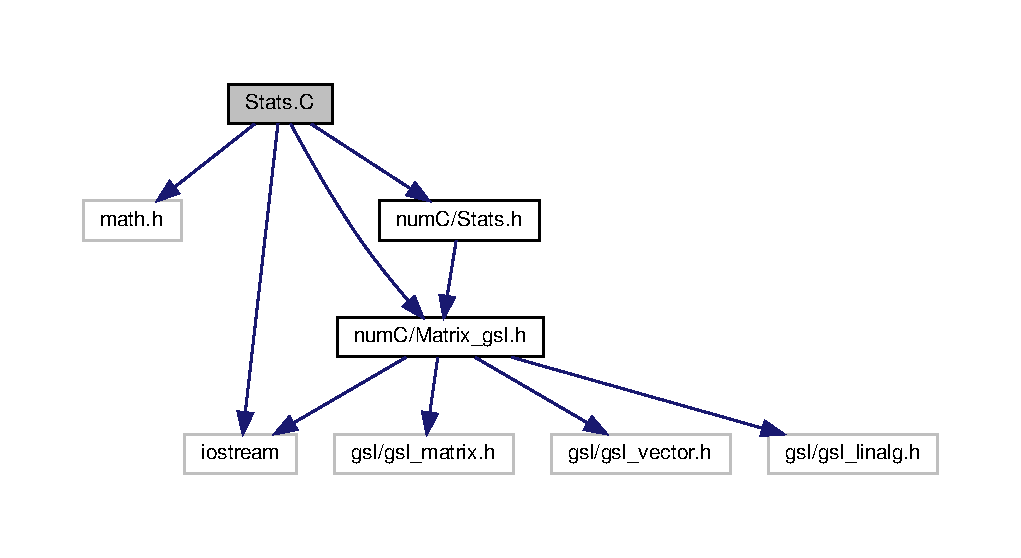
\includegraphics[width=350pt]{Stats_8C__incl}
\end{center}
\end{figure}
\subsubsection*{Functions}
\begin{DoxyCompactItemize}
\item 
\hyperlink{classMatrix}{Matrix} \hyperlink{Stats_8C_ae39b64f2f2f119f1fd195d6ca0583a6f}{ave} (\hyperlink{classMatrix}{Matrix} A, int axis)
\begin{DoxyCompactList}\small\item\em \hyperlink{classMatrix}{Matrix} average. \end{DoxyCompactList}\item 
\hyperlink{classMatrix}{Matrix} \hyperlink{Stats_8C_a2e68f0f11b60ca80c496e3afb4b7cc01}{var} (\hyperlink{classMatrix}{Matrix} A, int axis)
\begin{DoxyCompactList}\small\item\em \hyperlink{classMatrix}{Matrix} variance. \end{DoxyCompactList}\item 
\hyperlink{classMatrix}{Matrix} \hyperlink{Stats_8C_ac9e2628dd0e3b331f9113cf8d731b10c}{cov} (\hyperlink{classMatrix}{Matrix} A, int axis)
\begin{DoxyCompactList}\small\item\em Covariance matrix. \end{DoxyCompactList}\item 
\hyperlink{classMatrix}{Matrix} $\ast$ \hyperlink{Stats_8C_a143c09048292af2563e2996d2c2f4922}{J\+K\+\_\+resample} (\hyperlink{classMatrix}{Matrix} A, int axis)
\begin{DoxyCompactList}\small\item\em Jackknife resample. \end{DoxyCompactList}\item 
\hyperlink{classMatrix}{Matrix} \hyperlink{Stats_8C_affd6f6d5163a812e041030361c401f90}{sample\+\_\+ave} (\hyperlink{classMatrix}{Matrix} $\ast$A, int l)
\begin{DoxyCompactList}\small\item\em Sample average. \end{DoxyCompactList}\item 
\hyperlink{classMatrix}{Matrix} \hyperlink{Stats_8C_a0285e96e7ca20265cc8af9eafc5bbb3b}{J\+K\+\_\+error} (\hyperlink{classMatrix}{Matrix} $\ast$A, int l)
\begin{DoxyCompactList}\small\item\em Jackknife standard deviation. \end{DoxyCompactList}\item 
\hyperlink{classMatrix}{Matrix} \hyperlink{Stats_8C_ae2e8a930a8ea255b6deb8f17f4d45206}{B\+S\+\_\+error} (\hyperlink{classMatrix}{Matrix} $\ast$A, int l)
\begin{DoxyCompactList}\small\item\em Bootstrap standard deviation. \end{DoxyCompactList}\item 
double \hyperlink{Stats_8C_acf58aad875a53a890de07e717fa561b9}{chisqr} (\hyperlink{classMatrix}{Matrix} y\+\_\+bar, \hyperlink{classMatrix}{Matrix} c\+\_\+inv, \hyperlink{classMatrix}{Matrix} f)
\begin{DoxyCompactList}\small\item\em Chi square. \end{DoxyCompactList}\end{DoxyCompactItemize}


\subsubsection{Detailed Description}
Statistics tools. 



\subsubsection{Function Documentation}
\mbox{\Hypertarget{Stats_8C_ae39b64f2f2f119f1fd195d6ca0583a6f}\label{Stats_8C_ae39b64f2f2f119f1fd195d6ca0583a6f}} 
\index{Stats.\+C@{Stats.\+C}!ave@{ave}}
\index{ave@{ave}!Stats.\+C@{Stats.\+C}}
\paragraph{\texorpdfstring{ave()}{ave()}}
{\footnotesize\ttfamily \hyperlink{classMatrix}{Matrix} ave (\begin{DoxyParamCaption}\item[{\hyperlink{classMatrix}{Matrix}}]{A,  }\item[{int}]{axis = {\ttfamily 1} }\end{DoxyParamCaption})}



\hyperlink{classMatrix}{Matrix} average. 

Calculate average along the given axis

Parameters\+: 
\begin{DoxyParams}{Parameters}
{\em A} & (\hyperlink{classMatrix}{Matrix}) \hyperlink{classMatrix}{Matrix} to calculate \\
\hline
{\em axis} & (int) axis to calculate default = 1\\
\hline
\end{DoxyParams}
Returns\+: \begin{DoxyReturn}{Returns}
result (\hyperlink{classMatrix}{Matrix}) a vector (collapsed \hyperlink{classMatrix}{Matrix})
\end{DoxyReturn}
Example\+:

B = ave(\+A, 0);

Tag\+: average vector matrix 

Definition at line 13 of file Stats.\+C.



Referenced by cov(), and var().


\begin{DoxyCode}
13                               \{
14   
15   \textcolor{keywordtype}{int} n = A.shape[0];
16   \textcolor{keywordtype}{int} m = A.shape[1];
17 
18   \textcolor{keywordflow}{if}(axis == 1)\{
19 
20     \hyperlink{classMatrix}{Matrix} result(n,1,\textcolor{stringliteral}{"ave"});
21 
22     \textcolor{keywordflow}{for}(\textcolor{keywordtype}{int} i=0;i<n;i++)\{
23       \textcolor{keywordflow}{for}(\textcolor{keywordtype}{int} j=0;j<m;j++)\{
24         result.matrix[i][0] += A.matrix[i][j]/(1.*m);
25       \}
26     \}
27     
28     \textcolor{keywordflow}{return} result;
29   \}
30   \textcolor{keywordflow}{else} \textcolor{keywordflow}{if} (axis == 0)\{
31     
32     \hyperlink{classMatrix}{Matrix} result(1,m);
33     
34     \textcolor{keywordflow}{for}(\textcolor{keywordtype}{int} i=0;i<n;i++)\{
35       \textcolor{keywordflow}{for}(\textcolor{keywordtype}{int} j=0;j<m;j++) result.matrix[0][j] += A.matrix[i][j]/(1.*n);
36     \}
37 
38     \textcolor{keywordflow}{return} result;
39   \}
40 \}
\end{DoxyCode}
\mbox{\Hypertarget{Stats_8C_ae2e8a930a8ea255b6deb8f17f4d45206}\label{Stats_8C_ae2e8a930a8ea255b6deb8f17f4d45206}} 
\index{Stats.\+C@{Stats.\+C}!B\+S\+\_\+error@{B\+S\+\_\+error}}
\index{B\+S\+\_\+error@{B\+S\+\_\+error}!Stats.\+C@{Stats.\+C}}
\paragraph{\texorpdfstring{B\+S\+\_\+error()}{BS\_error()}}
{\footnotesize\ttfamily \hyperlink{classMatrix}{Matrix} B\+S\+\_\+error (\begin{DoxyParamCaption}\item[{\hyperlink{classMatrix}{Matrix} $\ast$}]{A,  }\item[{int}]{l }\end{DoxyParamCaption})}



Bootstrap standard deviation. 

Calculate standard deviation(sqrt(var), error) of Bootstrap resampled data

Parameters\+: 
\begin{DoxyParams}{Parameters}
{\em A} & (Matrix$\ast$) Bootstrap resampled data \\
\hline
{\em l} & (int) number of BS samples\\
\hline
\end{DoxyParams}
Returns\+: \begin{DoxyReturn}{Returns}
result (Martix) collapsed array of Matrices
\end{DoxyReturn}
Example\+:

A = B\+S\+\_\+error(\+B, 500);

Tag\+: Bootstrap standard deviation error 

Definition at line 163 of file Stats.\+C.



References sample\+\_\+ave().


\begin{DoxyCode}
163                                  \{
164   \textcolor{keywordtype}{int} n = A[0].shape[0];
165   
166   \hyperlink{classMatrix}{Matrix} A\_ave(n,1);
167   A\_ave = \hyperlink{Stats_8C_affd6f6d5163a812e041030361c401f90}{sample\_ave}(A, l);
168 
169   \hyperlink{classMatrix}{Matrix} result(n,1);
170 
171   \textcolor{keywordflow}{for}(\textcolor{keywordtype}{int} i=0;i<n;i++)\{
172     \textcolor{keywordflow}{for}(\textcolor{keywordtype}{int} j=0;j<l;j++) result.matrix[i][0] += pow(A[j].matrix[i][0] - A\_ave.matrix[i][0],2.) / (l-1.);
173   \}
174 
175   \textcolor{keywordflow}{for}(\textcolor{keywordtype}{int} i=0;i<n;i++) result.matrix[i][0] = sqrt(result.matrix[i][0]);
176 
177   \textcolor{keywordflow}{return} result;
178 \}
\end{DoxyCode}
\mbox{\Hypertarget{Stats_8C_acf58aad875a53a890de07e717fa561b9}\label{Stats_8C_acf58aad875a53a890de07e717fa561b9}} 
\index{Stats.\+C@{Stats.\+C}!chisqr@{chisqr}}
\index{chisqr@{chisqr}!Stats.\+C@{Stats.\+C}}
\paragraph{\texorpdfstring{chisqr()}{chisqr()}}
{\footnotesize\ttfamily double chisqr (\begin{DoxyParamCaption}\item[{\hyperlink{classMatrix}{Matrix}}]{y\+\_\+bar,  }\item[{\hyperlink{classMatrix}{Matrix}}]{c\+\_\+inv,  }\item[{\hyperlink{classMatrix}{Matrix}}]{f }\end{DoxyParamCaption})}



Chi square. 

Calculate chi-\/square of given data chi$^\wedge$2 = (y\+\_\+bar -\/ f)$^\wedge$T C$^\wedge$-\/1 (y\+\_\+bar -\/ f)

Parameters\+: 
\begin{DoxyParams}{Parameters}
{\em y\+\_\+bar} & (\hyperlink{classMatrix}{Matrix}) vector containing an average of the data \\
\hline
{\em c\+\_\+inv} & (\hyperlink{classMatrix}{Matrix}) inverse of covariance matrix \\
\hline
{\em f} & (\hyperlink{classMatrix}{Matrix}) vector of fitting function values\\
\hline
\end{DoxyParams}
Returns\+: \begin{DoxyReturn}{Returns}
result (double) chi$^\wedge$2 of given data and fitting function
\end{DoxyReturn}
Example\+:

chisq = chiqr(\+Y\+\_\+bar, C\+\_\+inv, F);

Tag\+: chi-\/square fitting 

Definition at line 180 of file Stats.\+C.



References matmul(), and sub().


\begin{DoxyCode}
180                                                    \{
181 
182   \textcolor{keywordtype}{double} result;
183 
184   result = \hyperlink{Matrix_8C_a74a9fe9c1d326c41a69926c97720f4d2}{matmul}(\hyperlink{Matrix_8C_a74a9fe9c1d326c41a69926c97720f4d2}{matmul}(\hyperlink{Matrix_8C_a238af1517ec23a6f0279ec5ee6364d6a}{sub}(y\_bar, f).T(), c\_inv), \hyperlink{Matrix_8C_a238af1517ec23a6f0279ec5ee6364d6a}{sub}(y\_bar, f)).matrix[0][0];
185 
186   \textcolor{keywordflow}{return} result;
187 \}
\end{DoxyCode}
\mbox{\Hypertarget{Stats_8C_ac9e2628dd0e3b331f9113cf8d731b10c}\label{Stats_8C_ac9e2628dd0e3b331f9113cf8d731b10c}} 
\index{Stats.\+C@{Stats.\+C}!cov@{cov}}
\index{cov@{cov}!Stats.\+C@{Stats.\+C}}
\paragraph{\texorpdfstring{cov()}{cov()}}
{\footnotesize\ttfamily \hyperlink{classMatrix}{Matrix} cov (\begin{DoxyParamCaption}\item[{\hyperlink{classMatrix}{Matrix}}]{A,  }\item[{int}]{axis = {\ttfamily 0} }\end{DoxyParamCaption})}



Covariance matrix. 

Calculate covariance along the given axis

Parameters\+: 
\begin{DoxyParams}{Parameters}
{\em A} & (\hyperlink{classMatrix}{Matrix}) \hyperlink{classMatrix}{Matrix} of data \\
\hline
{\em axis} & (int) axis to calculate default = 0\\
\hline
\end{DoxyParams}
Returns\+: \begin{DoxyReturn}{Returns}
result (\hyperlink{classMatrix}{Matrix}) covariance of vectors along axis
\end{DoxyReturn}
Example\+:

C = cov(\+A, 0);

Tag\+: covariance vector matrix 

Definition at line 70 of file Stats.\+C.



References ave().


\begin{DoxyCode}
70                               \{
71   \textcolor{comment}{// Default : sample covariance}
72 
73   \textcolor{keywordtype}{int} n = A.shape[0];
74   \textcolor{keywordtype}{int} m = A.shape[1];
75   
76   \textcolor{keywordflow}{if}(axis == 0)\{
77     \hyperlink{classMatrix}{Matrix} A\_ave;
78     A\_ave = \hyperlink{Stats_8C_ae39b64f2f2f119f1fd195d6ca0583a6f}{ave}(A, 1);
79 
80     \hyperlink{classMatrix}{Matrix} result(n,n);
81 
82     \textcolor{keywordflow}{for}(\textcolor{keywordtype}{int} i=0;i<n;i++)\{
83       \textcolor{keywordflow}{for}(\textcolor{keywordtype}{int} j=0;j<n;j++)\{
84         \textcolor{keywordflow}{for}(\textcolor{keywordtype}{int} k=0;k<m;k++)\{
85           result.matrix[i][j] += (A.matrix[i][k] - A\_ave.matrix[i][0]) * (A.matrix[j][k] - A\_ave.matrix[j][
      0])/(1.*m)/(m-1.);
86         \}
87       \}
88     \}
89 
90     \textcolor{keywordflow}{return} result;
91   \}
92   \textcolor{keywordflow}{else} \textcolor{keywordflow}{if}(axis == 1)\{
93     \hyperlink{classMatrix}{Matrix} A\_ave = \hyperlink{Stats_8C_ae39b64f2f2f119f1fd195d6ca0583a6f}{ave}(A, 0);
94 
95     \hyperlink{classMatrix}{Matrix} result(m,m);
96 
97     \textcolor{keywordflow}{for}(\textcolor{keywordtype}{int} i=0;i<m;i++)\{
98       \textcolor{keywordflow}{for}(\textcolor{keywordtype}{int} j=0;j<m;j++)\{
99         \textcolor{keywordflow}{for}(\textcolor{keywordtype}{int} k=0;k<n;k++) result.matrix[i][j] += (A.matrix[k][i] - A\_ave.matrix[0][i]) * (A.matrix[k][j]
       - A\_ave.matrix[0][j])/(1.*m)/(m-1.);
100       \}
101     \}
102 
103     \textcolor{keywordflow}{return} result;
104   \}
105 \}
\end{DoxyCode}
\mbox{\Hypertarget{Stats_8C_a0285e96e7ca20265cc8af9eafc5bbb3b}\label{Stats_8C_a0285e96e7ca20265cc8af9eafc5bbb3b}} 
\index{Stats.\+C@{Stats.\+C}!J\+K\+\_\+error@{J\+K\+\_\+error}}
\index{J\+K\+\_\+error@{J\+K\+\_\+error}!Stats.\+C@{Stats.\+C}}
\paragraph{\texorpdfstring{J\+K\+\_\+error()}{JK\_error()}}
{\footnotesize\ttfamily \hyperlink{classMatrix}{Matrix} J\+K\+\_\+error (\begin{DoxyParamCaption}\item[{\hyperlink{classMatrix}{Matrix} $\ast$}]{A,  }\item[{int}]{l }\end{DoxyParamCaption})}



Jackknife standard deviation. 

Calculate standard deviation(sqrt(var), error) of Jackknife resampled data

Parameters\+: 
\begin{DoxyParams}{Parameters}
{\em A} & (Matrix$\ast$) Jackknife resampled data \\
\hline
{\em l} & (int) number of JK samples (N)\\
\hline
\end{DoxyParams}
Returns\+: \begin{DoxyReturn}{Returns}
result (\hyperlink{classMatrix}{Matrix}) collapsed array of Matrices
\end{DoxyReturn}
Example\+:

A = J\+K\+\_\+error(\+B, 200);

Tag\+: Jackknife standard deviation error 

Definition at line 145 of file Stats.\+C.



References sample\+\_\+ave().


\begin{DoxyCode}
145                                  \{
146 
147   \textcolor{keywordtype}{int} n = A[0].shape[0];
148   
149   \hyperlink{classMatrix}{Matrix} A\_ave(n,1);
150   A\_ave = \hyperlink{Stats_8C_affd6f6d5163a812e041030361c401f90}{sample\_ave}(A, l);
151 
152   \hyperlink{classMatrix}{Matrix} result(n, 1);
153 
154   \textcolor{keywordflow}{for}(\textcolor{keywordtype}{int} i=0;i<n;i++)\{
155     \textcolor{keywordflow}{for}(\textcolor{keywordtype}{int} j=0;j<l;j++) result.matrix[i][0] += pow(A[j].matrix[i][0] - A\_ave.matrix[i][0], 2.) /(1.*l)*(l-
      1.);
156   \}
157 
158   \textcolor{keywordflow}{for}(\textcolor{keywordtype}{int} i=0;i<n;i++) result.matrix[i][0] = sqrt(result.matrix[i][0]);
159 
160   \textcolor{keywordflow}{return} result;
161 \}
\end{DoxyCode}
\mbox{\Hypertarget{Stats_8C_a143c09048292af2563e2996d2c2f4922}\label{Stats_8C_a143c09048292af2563e2996d2c2f4922}} 
\index{Stats.\+C@{Stats.\+C}!J\+K\+\_\+resample@{J\+K\+\_\+resample}}
\index{J\+K\+\_\+resample@{J\+K\+\_\+resample}!Stats.\+C@{Stats.\+C}}
\paragraph{\texorpdfstring{J\+K\+\_\+resample()}{JK\_resample()}}
{\footnotesize\ttfamily \hyperlink{classMatrix}{Matrix}$\ast$ J\+K\+\_\+resample (\begin{DoxyParamCaption}\item[{\hyperlink{classMatrix}{Matrix}}]{A,  }\item[{int}]{axis = {\ttfamily 1} }\end{DoxyParamCaption})}



Jackknife resample. 

Resample along the given axis It samples maximum amount of data (N samples)

Parameters\+: 
\begin{DoxyParams}{Parameters}
{\em A} & (\hyperlink{classMatrix}{Matrix}) \hyperlink{classMatrix}{Matrix} of data \\
\hline
{\em axis} & (int) axis to calculate default = 1\\
\hline
\end{DoxyParams}
Returns\+: \begin{DoxyReturn}{Returns}
result (Matrix$\ast$) Array(\+Pointer) of matrix
\end{DoxyReturn}
Example\+:

X = J\+K\+\_\+resample(\+A, 0);

Tag\+: Jackknife resampling 

Definition at line 107 of file Stats.\+C.


\begin{DoxyCode}
107                                        \{
108   
109   \textcolor{keywordtype}{int} n = A.shape[0];
110   \textcolor{keywordtype}{int} m = A.shape[1];
111 
112   \hyperlink{classMatrix}{Matrix} *result;
113   result = \textcolor{keyword}{new} \hyperlink{classMatrix}{Matrix} [m];
114   \textcolor{keywordflow}{for}(\textcolor{keywordtype}{int} i=0;i<m;i++) result[i].init(n, m-1);
115 
116   \textcolor{keywordtype}{int} p=0;
117   \textcolor{keywordflow}{for}(\textcolor{keywordtype}{int} i=0;i<m;i++)\{
118     \textcolor{keywordflow}{for}(\textcolor{keywordtype}{int} j=0;j<n;j++)\{
119       p = 0;
120       \textcolor{keywordflow}{for}(\textcolor{keywordtype}{int} k=0;k<m;k++)\{
121         \textcolor{keywordflow}{if}(i != k)\{
122           result[i].matrix[j][p] = A.matrix[j][k];
123           p++;
124         \}
125       \}
126     \}
127   \}
128 
129   \textcolor{keywordflow}{return} result;
130 \}
\end{DoxyCode}
\mbox{\Hypertarget{Stats_8C_affd6f6d5163a812e041030361c401f90}\label{Stats_8C_affd6f6d5163a812e041030361c401f90}} 
\index{Stats.\+C@{Stats.\+C}!sample\+\_\+ave@{sample\+\_\+ave}}
\index{sample\+\_\+ave@{sample\+\_\+ave}!Stats.\+C@{Stats.\+C}}
\paragraph{\texorpdfstring{sample\+\_\+ave()}{sample\_ave()}}
{\footnotesize\ttfamily \hyperlink{classMatrix}{Matrix} sample\+\_\+ave (\begin{DoxyParamCaption}\item[{\hyperlink{classMatrix}{Matrix} $\ast$}]{A,  }\item[{int}]{l }\end{DoxyParamCaption})}



Sample average. 

Calculate average of array(pointer) of Matrices

Parameters\+: 
\begin{DoxyParams}{Parameters}
{\em A} & (Matrix$\ast$) Pointer to \hyperlink{classMatrix}{Matrix} eg) resampled data \\
\hline
{\em l} & (int) number of JK samples (N)\\
\hline
\end{DoxyParams}
Returns\+: \begin{DoxyReturn}{Returns}
result (\hyperlink{classMatrix}{Matrix}) collapsed array of Matrices
\end{DoxyReturn}
Example\+:

A = sample\+\_\+ave(\+B, 200);

Tag\+: Jackknife average 

Definition at line 132 of file Stats.\+C.



Referenced by B\+S\+\_\+error(), and J\+K\+\_\+error().


\begin{DoxyCode}
132                                    \{
133 
134   \textcolor{keywordtype}{int} n = A[0].shape[0];
135 
136   \hyperlink{classMatrix}{Matrix} result(n,1);
137 
138   \textcolor{keywordflow}{for}(\textcolor{keywordtype}{int} i=0;i<n;i++)\{
139     \textcolor{keywordflow}{for}(\textcolor{keywordtype}{int} j=0;j<l;j++) result.matrix[i][0] += A[j].matrix[i][0]/(1.*l);
140   \}
141 
142   \textcolor{keywordflow}{return} result;
143 \}
\end{DoxyCode}
\mbox{\Hypertarget{Stats_8C_a2e68f0f11b60ca80c496e3afb4b7cc01}\label{Stats_8C_a2e68f0f11b60ca80c496e3afb4b7cc01}} 
\index{Stats.\+C@{Stats.\+C}!var@{var}}
\index{var@{var}!Stats.\+C@{Stats.\+C}}
\paragraph{\texorpdfstring{var()}{var()}}
{\footnotesize\ttfamily \hyperlink{classMatrix}{Matrix} var (\begin{DoxyParamCaption}\item[{\hyperlink{classMatrix}{Matrix}}]{A,  }\item[{int}]{axis = {\ttfamily 1} }\end{DoxyParamCaption})}



\hyperlink{classMatrix}{Matrix} variance. 

Calculate variance along the given axis

Parameters\+: 
\begin{DoxyParams}{Parameters}
{\em A} & (\hyperlink{classMatrix}{Matrix}) \hyperlink{classMatrix}{Matrix} to calculate \\
\hline
{\em axis} & (int) axis to calculate default = 1\\
\hline
\end{DoxyParams}
Returns\+: \begin{DoxyReturn}{Returns}
result (\hyperlink{classMatrix}{Matrix}) a vector (collapsed \hyperlink{classMatrix}{Matrix})
\end{DoxyReturn}
Example\+:

B = var(\+A,0);

Tag\+: variance vector matrix 

Definition at line 42 of file Stats.\+C.



References ave().


\begin{DoxyCode}
42                               \{
43   \textcolor{comment}{// Default : sample var}
44 
45   \textcolor{keywordtype}{int} n = A.shape[0];
46   \textcolor{keywordtype}{int} m = A.shape[1];
47 
48   \textcolor{keywordflow}{if}(axis == 1)\{
49     \hyperlink{classMatrix}{Matrix} A\_ave = \hyperlink{Stats_8C_ae39b64f2f2f119f1fd195d6ca0583a6f}{ave}(A, 1);
50     \hyperlink{classMatrix}{Matrix} result(n,1);
51 
52     \textcolor{keywordflow}{for}(\textcolor{keywordtype}{int} i=0;i<n;i++)\{
53       \textcolor{keywordflow}{for}(\textcolor{keywordtype}{int} j=0;j<m;j++) result.matrix[i][0] += pow(A.matrix[i][j] - A\_ave.matrix[i][0], 2.)/(1.*m)/(m - 
      1.);
54     \}
55 
56     \textcolor{keywordflow}{return} result;
57   \}
58   \textcolor{keywordflow}{else} \textcolor{keywordflow}{if}(axis == 0)\{
59     \hyperlink{classMatrix}{Matrix} A\_ave = \hyperlink{Stats_8C_ae39b64f2f2f119f1fd195d6ca0583a6f}{ave}(A, 0);
60     \hyperlink{classMatrix}{Matrix} result(1,m);
61     
62     \textcolor{keywordflow}{for}(\textcolor{keywordtype}{int} i=0;i<n;i++)\{
63       \textcolor{keywordflow}{for}(\textcolor{keywordtype}{int} j=0;j<m;j++) result.matrix[0][j] += pow(A.matrix[i][j] - A\_ave.matrix[0][j], 2.)/(1.*n)/(n - 
      1.);
64     \}
65 
66     \textcolor{keywordflow}{return} result;
67   \}
68 \}
\end{DoxyCode}

\hypertarget{Stats_8h}{}\subsection{Stats.\+h File Reference}
\label{Stats_8h}\index{Stats.\+h@{Stats.\+h}}


Statistics tools.  


{\ttfamily \#include $<$num\+C/\+Matrix\+\_\+gsl.\+h$>$}\newline
Include dependency graph for Stats.\+h\+:
\nopagebreak
\begin{figure}[H]
\begin{center}
\leavevmode
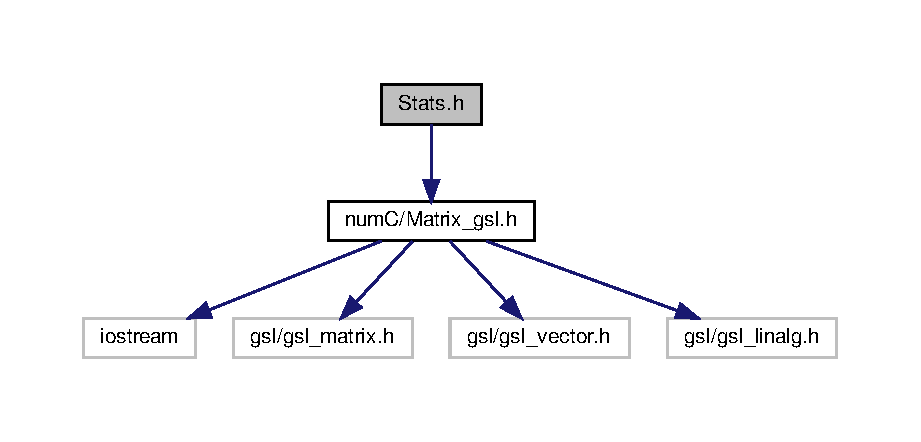
\includegraphics[width=350pt]{Stats_8h__incl}
\end{center}
\end{figure}
This graph shows which files directly or indirectly include this file\+:
\nopagebreak
\begin{figure}[H]
\begin{center}
\leavevmode
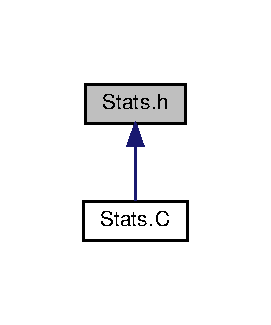
\includegraphics[width=130pt]{Stats_8h__dep__incl}
\end{center}
\end{figure}
\subsubsection*{Functions}
\begin{DoxyCompactItemize}
\item 
\hyperlink{classMatrix}{Matrix} \hyperlink{Stats_8h_ad57e6830355961246be2c949907bb4eb}{ave} (\hyperlink{classMatrix}{Matrix} A, int axis=1)
\begin{DoxyCompactList}\small\item\em \hyperlink{classMatrix}{Matrix} average. \end{DoxyCompactList}\item 
\hyperlink{classMatrix}{Matrix} \hyperlink{Stats_8h_ac513281436df47e26cb6fc01634cf28a}{var} (\hyperlink{classMatrix}{Matrix} A, int axis=1)
\begin{DoxyCompactList}\small\item\em \hyperlink{classMatrix}{Matrix} variance. \end{DoxyCompactList}\item 
\hyperlink{classMatrix}{Matrix} \hyperlink{Stats_8h_adcae8e0ffa58204a0438aed644fb3937}{cov} (\hyperlink{classMatrix}{Matrix} A, int axis=0)
\begin{DoxyCompactList}\small\item\em Covariance matrix. \end{DoxyCompactList}\item 
\hyperlink{classMatrix}{Matrix} $\ast$ \hyperlink{Stats_8h_a7195a46887f9beaaac1bc5238818ef64}{J\+K\+\_\+resample} (\hyperlink{classMatrix}{Matrix} A, int axis=1)
\begin{DoxyCompactList}\small\item\em Jackknife resample. \end{DoxyCompactList}\item 
\hyperlink{classMatrix}{Matrix} \hyperlink{Stats_8h_affd6f6d5163a812e041030361c401f90}{sample\+\_\+ave} (\hyperlink{classMatrix}{Matrix} $\ast$A, int l)
\begin{DoxyCompactList}\small\item\em Sample average. \end{DoxyCompactList}\item 
\hyperlink{classMatrix}{Matrix} \hyperlink{Stats_8h_a0285e96e7ca20265cc8af9eafc5bbb3b}{J\+K\+\_\+error} (\hyperlink{classMatrix}{Matrix} $\ast$A, int l)
\begin{DoxyCompactList}\small\item\em Jackknife standard deviation. \end{DoxyCompactList}\item 
\hyperlink{classMatrix}{Matrix} \hyperlink{Stats_8h_ae2e8a930a8ea255b6deb8f17f4d45206}{B\+S\+\_\+error} (\hyperlink{classMatrix}{Matrix} $\ast$A, int l)
\begin{DoxyCompactList}\small\item\em Bootstrap standard deviation. \end{DoxyCompactList}\item 
double \hyperlink{Stats_8h_acf58aad875a53a890de07e717fa561b9}{chisqr} (\hyperlink{classMatrix}{Matrix} y\+\_\+bar, \hyperlink{classMatrix}{Matrix} c\+\_\+inv, \hyperlink{classMatrix}{Matrix} f)
\begin{DoxyCompactList}\small\item\em Chi square. \end{DoxyCompactList}\end{DoxyCompactItemize}


\subsubsection{Detailed Description}
Statistics tools. 

\begin{DoxyDate}{Date}
Nov 22, 2021 
\end{DoxyDate}
\begin{DoxyAuthor}{Author}
C J Park ~\newline
 \href{mailto:chanjure@snu.ac.kr}{\tt chanjure@snu.\+ac.\+kr} 
\end{DoxyAuthor}
\begin{DoxyRefDesc}{Bug}
\item[\hyperlink{bug__bug000002}{Bug}]No known bugs. \end{DoxyRefDesc}
\begin{DoxyVersion}{Version}
1.\+0 
\end{DoxyVersion}


\subsubsection{Function Documentation}
\mbox{\Hypertarget{Stats_8h_ad57e6830355961246be2c949907bb4eb}\label{Stats_8h_ad57e6830355961246be2c949907bb4eb}} 
\index{Stats.\+h@{Stats.\+h}!ave@{ave}}
\index{ave@{ave}!Stats.\+h@{Stats.\+h}}
\paragraph{\texorpdfstring{ave()}{ave()}}
{\footnotesize\ttfamily \hyperlink{classMatrix}{Matrix} ave (\begin{DoxyParamCaption}\item[{\hyperlink{classMatrix}{Matrix}}]{A,  }\item[{int}]{axis = {\ttfamily 1} }\end{DoxyParamCaption})}



\hyperlink{classMatrix}{Matrix} average. 

Calculate average along the given axis

Parameters\+: 
\begin{DoxyParams}{Parameters}
{\em A} & (\hyperlink{classMatrix}{Matrix}) \hyperlink{classMatrix}{Matrix} to calculate \\
\hline
{\em axis} & (int) axis to calculate default = 1\\
\hline
\end{DoxyParams}
Returns\+: \begin{DoxyReturn}{Returns}
result (\hyperlink{classMatrix}{Matrix}) a vector (collapsed \hyperlink{classMatrix}{Matrix})
\end{DoxyReturn}
Example\+:

B = ave(\+A, 0);

Tag\+: average vector matrix 

Definition at line 13 of file Stats.\+C.



Referenced by cov(), and var().


\begin{DoxyCode}
13                               \{
14   
15   \textcolor{keywordtype}{int} n = A.shape[0];
16   \textcolor{keywordtype}{int} m = A.shape[1];
17 
18   \textcolor{keywordflow}{if}(axis == 1)\{
19 
20     \hyperlink{classMatrix}{Matrix} result(n,1,\textcolor{stringliteral}{"ave"});
21 
22     \textcolor{keywordflow}{for}(\textcolor{keywordtype}{int} i=0;i<n;i++)\{
23       \textcolor{keywordflow}{for}(\textcolor{keywordtype}{int} j=0;j<m;j++)\{
24         result.matrix[i][0] += A.matrix[i][j]/(1.*m);
25       \}
26     \}
27     
28     \textcolor{keywordflow}{return} result;
29   \}
30   \textcolor{keywordflow}{else} \textcolor{keywordflow}{if} (axis == 0)\{
31     
32     \hyperlink{classMatrix}{Matrix} result(1,m);
33     
34     \textcolor{keywordflow}{for}(\textcolor{keywordtype}{int} i=0;i<n;i++)\{
35       \textcolor{keywordflow}{for}(\textcolor{keywordtype}{int} j=0;j<m;j++) result.matrix[0][j] += A.matrix[i][j]/(1.*n);
36     \}
37 
38     \textcolor{keywordflow}{return} result;
39   \}
40 \}
\end{DoxyCode}
\mbox{\Hypertarget{Stats_8h_ae2e8a930a8ea255b6deb8f17f4d45206}\label{Stats_8h_ae2e8a930a8ea255b6deb8f17f4d45206}} 
\index{Stats.\+h@{Stats.\+h}!B\+S\+\_\+error@{B\+S\+\_\+error}}
\index{B\+S\+\_\+error@{B\+S\+\_\+error}!Stats.\+h@{Stats.\+h}}
\paragraph{\texorpdfstring{B\+S\+\_\+error()}{BS\_error()}}
{\footnotesize\ttfamily \hyperlink{classMatrix}{Matrix} B\+S\+\_\+error (\begin{DoxyParamCaption}\item[{\hyperlink{classMatrix}{Matrix} $\ast$}]{A,  }\item[{int}]{l }\end{DoxyParamCaption})}



Bootstrap standard deviation. 

Calculate standard deviation(sqrt(var), error) of Bootstrap resampled data

Parameters\+: 
\begin{DoxyParams}{Parameters}
{\em A} & (Matrix$\ast$) Bootstrap resampled data \\
\hline
{\em l} & (int) number of BS samples\\
\hline
\end{DoxyParams}
Returns\+: \begin{DoxyReturn}{Returns}
result (Martix) collapsed array of Matrices
\end{DoxyReturn}
Example\+:

A = B\+S\+\_\+error(\+B, 500);

Tag\+: Bootstrap standard deviation error 

Definition at line 163 of file Stats.\+C.



References sample\+\_\+ave().


\begin{DoxyCode}
163                                  \{
164   \textcolor{keywordtype}{int} n = A[0].shape[0];
165   
166   \hyperlink{classMatrix}{Matrix} A\_ave(n,1);
167   A\_ave = \hyperlink{Stats_8C_affd6f6d5163a812e041030361c401f90}{sample\_ave}(A, l);
168 
169   \hyperlink{classMatrix}{Matrix} result(n,1);
170 
171   \textcolor{keywordflow}{for}(\textcolor{keywordtype}{int} i=0;i<n;i++)\{
172     \textcolor{keywordflow}{for}(\textcolor{keywordtype}{int} j=0;j<l;j++) result.matrix[i][0] += pow(A[j].matrix[i][0] - A\_ave.matrix[i][0],2.) / (l-1.);
173   \}
174 
175   \textcolor{keywordflow}{for}(\textcolor{keywordtype}{int} i=0;i<n;i++) result.matrix[i][0] = sqrt(result.matrix[i][0]);
176 
177   \textcolor{keywordflow}{return} result;
178 \}
\end{DoxyCode}
\mbox{\Hypertarget{Stats_8h_acf58aad875a53a890de07e717fa561b9}\label{Stats_8h_acf58aad875a53a890de07e717fa561b9}} 
\index{Stats.\+h@{Stats.\+h}!chisqr@{chisqr}}
\index{chisqr@{chisqr}!Stats.\+h@{Stats.\+h}}
\paragraph{\texorpdfstring{chisqr()}{chisqr()}}
{\footnotesize\ttfamily double chisqr (\begin{DoxyParamCaption}\item[{\hyperlink{classMatrix}{Matrix}}]{y\+\_\+bar,  }\item[{\hyperlink{classMatrix}{Matrix}}]{c\+\_\+inv,  }\item[{\hyperlink{classMatrix}{Matrix}}]{f }\end{DoxyParamCaption})}



Chi square. 

Calculate chi-\/square of given data chi$^\wedge$2 = (y\+\_\+bar -\/ f)$^\wedge$T C$^\wedge$-\/1 (y\+\_\+bar -\/ f)

Parameters\+: 
\begin{DoxyParams}{Parameters}
{\em y\+\_\+bar} & (\hyperlink{classMatrix}{Matrix}) vector containing an average of the data \\
\hline
{\em c\+\_\+inv} & (\hyperlink{classMatrix}{Matrix}) inverse of covariance matrix \\
\hline
{\em f} & (\hyperlink{classMatrix}{Matrix}) vector of fitting function values\\
\hline
\end{DoxyParams}
Returns\+: \begin{DoxyReturn}{Returns}
result (double) chi$^\wedge$2 of given data and fitting function
\end{DoxyReturn}
Example\+:

chisq = chiqr(\+Y\+\_\+bar, C\+\_\+inv, F);

Tag\+: chi-\/square fitting 

Definition at line 180 of file Stats.\+C.



References matmul(), and sub().


\begin{DoxyCode}
180                                                    \{
181 
182   \textcolor{keywordtype}{double} result;
183 
184   result = \hyperlink{Matrix_8C_a74a9fe9c1d326c41a69926c97720f4d2}{matmul}(\hyperlink{Matrix_8C_a74a9fe9c1d326c41a69926c97720f4d2}{matmul}(\hyperlink{Matrix_8C_a238af1517ec23a6f0279ec5ee6364d6a}{sub}(y\_bar, f).T(), c\_inv), \hyperlink{Matrix_8C_a238af1517ec23a6f0279ec5ee6364d6a}{sub}(y\_bar, f)).matrix[0][0];
185 
186   \textcolor{keywordflow}{return} result;
187 \}
\end{DoxyCode}
\mbox{\Hypertarget{Stats_8h_adcae8e0ffa58204a0438aed644fb3937}\label{Stats_8h_adcae8e0ffa58204a0438aed644fb3937}} 
\index{Stats.\+h@{Stats.\+h}!cov@{cov}}
\index{cov@{cov}!Stats.\+h@{Stats.\+h}}
\paragraph{\texorpdfstring{cov()}{cov()}}
{\footnotesize\ttfamily \hyperlink{classMatrix}{Matrix} cov (\begin{DoxyParamCaption}\item[{\hyperlink{classMatrix}{Matrix}}]{A,  }\item[{int}]{axis = {\ttfamily 0} }\end{DoxyParamCaption})}



Covariance matrix. 

Calculate covariance along the given axis

Parameters\+: 
\begin{DoxyParams}{Parameters}
{\em A} & (\hyperlink{classMatrix}{Matrix}) \hyperlink{classMatrix}{Matrix} of data \\
\hline
{\em axis} & (int) axis to calculate default = 0\\
\hline
\end{DoxyParams}
Returns\+: \begin{DoxyReturn}{Returns}
result (\hyperlink{classMatrix}{Matrix}) covariance of vectors along axis
\end{DoxyReturn}
Example\+:

C = cov(\+A, 0);

Tag\+: covariance vector matrix 

Definition at line 70 of file Stats.\+C.



References ave().


\begin{DoxyCode}
70                               \{
71   \textcolor{comment}{// Default : sample covariance}
72 
73   \textcolor{keywordtype}{int} n = A.shape[0];
74   \textcolor{keywordtype}{int} m = A.shape[1];
75   
76   \textcolor{keywordflow}{if}(axis == 0)\{
77     \hyperlink{classMatrix}{Matrix} A\_ave;
78     A\_ave = \hyperlink{Stats_8C_ae39b64f2f2f119f1fd195d6ca0583a6f}{ave}(A, 1);
79 
80     \hyperlink{classMatrix}{Matrix} result(n,n);
81 
82     \textcolor{keywordflow}{for}(\textcolor{keywordtype}{int} i=0;i<n;i++)\{
83       \textcolor{keywordflow}{for}(\textcolor{keywordtype}{int} j=0;j<n;j++)\{
84         \textcolor{keywordflow}{for}(\textcolor{keywordtype}{int} k=0;k<m;k++)\{
85           result.matrix[i][j] += (A.matrix[i][k] - A\_ave.matrix[i][0]) * (A.matrix[j][k] - A\_ave.matrix[j][
      0])/(1.*m)/(m-1.);
86         \}
87       \}
88     \}
89 
90     \textcolor{keywordflow}{return} result;
91   \}
92   \textcolor{keywordflow}{else} \textcolor{keywordflow}{if}(axis == 1)\{
93     \hyperlink{classMatrix}{Matrix} A\_ave = \hyperlink{Stats_8C_ae39b64f2f2f119f1fd195d6ca0583a6f}{ave}(A, 0);
94 
95     \hyperlink{classMatrix}{Matrix} result(m,m);
96 
97     \textcolor{keywordflow}{for}(\textcolor{keywordtype}{int} i=0;i<m;i++)\{
98       \textcolor{keywordflow}{for}(\textcolor{keywordtype}{int} j=0;j<m;j++)\{
99         \textcolor{keywordflow}{for}(\textcolor{keywordtype}{int} k=0;k<n;k++) result.matrix[i][j] += (A.matrix[k][i] - A\_ave.matrix[0][i]) * (A.matrix[k][j]
       - A\_ave.matrix[0][j])/(1.*m)/(m-1.);
100       \}
101     \}
102 
103     \textcolor{keywordflow}{return} result;
104   \}
105 \}
\end{DoxyCode}
\mbox{\Hypertarget{Stats_8h_a0285e96e7ca20265cc8af9eafc5bbb3b}\label{Stats_8h_a0285e96e7ca20265cc8af9eafc5bbb3b}} 
\index{Stats.\+h@{Stats.\+h}!J\+K\+\_\+error@{J\+K\+\_\+error}}
\index{J\+K\+\_\+error@{J\+K\+\_\+error}!Stats.\+h@{Stats.\+h}}
\paragraph{\texorpdfstring{J\+K\+\_\+error()}{JK\_error()}}
{\footnotesize\ttfamily \hyperlink{classMatrix}{Matrix} J\+K\+\_\+error (\begin{DoxyParamCaption}\item[{\hyperlink{classMatrix}{Matrix} $\ast$}]{A,  }\item[{int}]{l }\end{DoxyParamCaption})}



Jackknife standard deviation. 

Calculate standard deviation(sqrt(var), error) of Jackknife resampled data

Parameters\+: 
\begin{DoxyParams}{Parameters}
{\em A} & (Matrix$\ast$) Jackknife resampled data \\
\hline
{\em l} & (int) number of JK samples (N)\\
\hline
\end{DoxyParams}
Returns\+: \begin{DoxyReturn}{Returns}
result (\hyperlink{classMatrix}{Matrix}) collapsed array of Matrices
\end{DoxyReturn}
Example\+:

A = J\+K\+\_\+error(\+B, 200);

Tag\+: Jackknife standard deviation error 

Definition at line 145 of file Stats.\+C.



References sample\+\_\+ave().


\begin{DoxyCode}
145                                  \{
146 
147   \textcolor{keywordtype}{int} n = A[0].shape[0];
148   
149   \hyperlink{classMatrix}{Matrix} A\_ave(n,1);
150   A\_ave = \hyperlink{Stats_8C_affd6f6d5163a812e041030361c401f90}{sample\_ave}(A, l);
151 
152   \hyperlink{classMatrix}{Matrix} result(n, 1);
153 
154   \textcolor{keywordflow}{for}(\textcolor{keywordtype}{int} i=0;i<n;i++)\{
155     \textcolor{keywordflow}{for}(\textcolor{keywordtype}{int} j=0;j<l;j++) result.matrix[i][0] += pow(A[j].matrix[i][0] - A\_ave.matrix[i][0], 2.) /(1.*l)*(l-
      1.);
156   \}
157 
158   \textcolor{keywordflow}{for}(\textcolor{keywordtype}{int} i=0;i<n;i++) result.matrix[i][0] = sqrt(result.matrix[i][0]);
159 
160   \textcolor{keywordflow}{return} result;
161 \}
\end{DoxyCode}
\mbox{\Hypertarget{Stats_8h_a7195a46887f9beaaac1bc5238818ef64}\label{Stats_8h_a7195a46887f9beaaac1bc5238818ef64}} 
\index{Stats.\+h@{Stats.\+h}!J\+K\+\_\+resample@{J\+K\+\_\+resample}}
\index{J\+K\+\_\+resample@{J\+K\+\_\+resample}!Stats.\+h@{Stats.\+h}}
\paragraph{\texorpdfstring{J\+K\+\_\+resample()}{JK\_resample()}}
{\footnotesize\ttfamily \hyperlink{classMatrix}{Matrix}$\ast$ J\+K\+\_\+resample (\begin{DoxyParamCaption}\item[{\hyperlink{classMatrix}{Matrix}}]{A,  }\item[{int}]{axis = {\ttfamily 1} }\end{DoxyParamCaption})}



Jackknife resample. 

Resample along the given axis It samples maximum amount of data (N samples)

Parameters\+: 
\begin{DoxyParams}{Parameters}
{\em A} & (\hyperlink{classMatrix}{Matrix}) \hyperlink{classMatrix}{Matrix} of data \\
\hline
{\em axis} & (int) axis to calculate default = 1\\
\hline
\end{DoxyParams}
Returns\+: \begin{DoxyReturn}{Returns}
result (Matrix$\ast$) Array(\+Pointer) of matrix
\end{DoxyReturn}
Example\+:

X = J\+K\+\_\+resample(\+A, 0);

Tag\+: Jackknife resampling 

Definition at line 107 of file Stats.\+C.


\begin{DoxyCode}
107                                        \{
108   
109   \textcolor{keywordtype}{int} n = A.shape[0];
110   \textcolor{keywordtype}{int} m = A.shape[1];
111 
112   \hyperlink{classMatrix}{Matrix} *result;
113   result = \textcolor{keyword}{new} \hyperlink{classMatrix}{Matrix} [m];
114   \textcolor{keywordflow}{for}(\textcolor{keywordtype}{int} i=0;i<m;i++) result[i].init(n, m-1);
115 
116   \textcolor{keywordtype}{int} p=0;
117   \textcolor{keywordflow}{for}(\textcolor{keywordtype}{int} i=0;i<m;i++)\{
118     \textcolor{keywordflow}{for}(\textcolor{keywordtype}{int} j=0;j<n;j++)\{
119       p = 0;
120       \textcolor{keywordflow}{for}(\textcolor{keywordtype}{int} k=0;k<m;k++)\{
121         \textcolor{keywordflow}{if}(i != k)\{
122           result[i].matrix[j][p] = A.matrix[j][k];
123           p++;
124         \}
125       \}
126     \}
127   \}
128 
129   \textcolor{keywordflow}{return} result;
130 \}
\end{DoxyCode}
\mbox{\Hypertarget{Stats_8h_affd6f6d5163a812e041030361c401f90}\label{Stats_8h_affd6f6d5163a812e041030361c401f90}} 
\index{Stats.\+h@{Stats.\+h}!sample\+\_\+ave@{sample\+\_\+ave}}
\index{sample\+\_\+ave@{sample\+\_\+ave}!Stats.\+h@{Stats.\+h}}
\paragraph{\texorpdfstring{sample\+\_\+ave()}{sample\_ave()}}
{\footnotesize\ttfamily \hyperlink{classMatrix}{Matrix} sample\+\_\+ave (\begin{DoxyParamCaption}\item[{\hyperlink{classMatrix}{Matrix} $\ast$}]{A,  }\item[{int}]{l }\end{DoxyParamCaption})}



Sample average. 

Calculate average of array(pointer) of Matrices

Parameters\+: 
\begin{DoxyParams}{Parameters}
{\em A} & (Matrix$\ast$) Pointer to \hyperlink{classMatrix}{Matrix} eg) resampled data \\
\hline
{\em l} & (int) number of JK samples (N)\\
\hline
\end{DoxyParams}
Returns\+: \begin{DoxyReturn}{Returns}
result (\hyperlink{classMatrix}{Matrix}) collapsed array of Matrices
\end{DoxyReturn}
Example\+:

A = sample\+\_\+ave(\+B, 200);

Tag\+: Jackknife average 

Definition at line 132 of file Stats.\+C.



Referenced by B\+S\+\_\+error(), and J\+K\+\_\+error().


\begin{DoxyCode}
132                                    \{
133 
134   \textcolor{keywordtype}{int} n = A[0].shape[0];
135 
136   \hyperlink{classMatrix}{Matrix} result(n,1);
137 
138   \textcolor{keywordflow}{for}(\textcolor{keywordtype}{int} i=0;i<n;i++)\{
139     \textcolor{keywordflow}{for}(\textcolor{keywordtype}{int} j=0;j<l;j++) result.matrix[i][0] += A[j].matrix[i][0]/(1.*l);
140   \}
141 
142   \textcolor{keywordflow}{return} result;
143 \}
\end{DoxyCode}
\mbox{\Hypertarget{Stats_8h_ac513281436df47e26cb6fc01634cf28a}\label{Stats_8h_ac513281436df47e26cb6fc01634cf28a}} 
\index{Stats.\+h@{Stats.\+h}!var@{var}}
\index{var@{var}!Stats.\+h@{Stats.\+h}}
\paragraph{\texorpdfstring{var()}{var()}}
{\footnotesize\ttfamily \hyperlink{classMatrix}{Matrix} var (\begin{DoxyParamCaption}\item[{\hyperlink{classMatrix}{Matrix}}]{A,  }\item[{int}]{axis = {\ttfamily 1} }\end{DoxyParamCaption})}



\hyperlink{classMatrix}{Matrix} variance. 

Calculate variance along the given axis

Parameters\+: 
\begin{DoxyParams}{Parameters}
{\em A} & (\hyperlink{classMatrix}{Matrix}) \hyperlink{classMatrix}{Matrix} to calculate \\
\hline
{\em axis} & (int) axis to calculate default = 1\\
\hline
\end{DoxyParams}
Returns\+: \begin{DoxyReturn}{Returns}
result (\hyperlink{classMatrix}{Matrix}) a vector (collapsed \hyperlink{classMatrix}{Matrix})
\end{DoxyReturn}
Example\+:

B = var(\+A,0);

Tag\+: variance vector matrix 

Definition at line 42 of file Stats.\+C.



References ave().


\begin{DoxyCode}
42                               \{
43   \textcolor{comment}{// Default : sample var}
44 
45   \textcolor{keywordtype}{int} n = A.shape[0];
46   \textcolor{keywordtype}{int} m = A.shape[1];
47 
48   \textcolor{keywordflow}{if}(axis == 1)\{
49     \hyperlink{classMatrix}{Matrix} A\_ave = \hyperlink{Stats_8C_ae39b64f2f2f119f1fd195d6ca0583a6f}{ave}(A, 1);
50     \hyperlink{classMatrix}{Matrix} result(n,1);
51 
52     \textcolor{keywordflow}{for}(\textcolor{keywordtype}{int} i=0;i<n;i++)\{
53       \textcolor{keywordflow}{for}(\textcolor{keywordtype}{int} j=0;j<m;j++) result.matrix[i][0] += pow(A.matrix[i][j] - A\_ave.matrix[i][0], 2.)/(1.*m)/(m - 
      1.);
54     \}
55 
56     \textcolor{keywordflow}{return} result;
57   \}
58   \textcolor{keywordflow}{else} \textcolor{keywordflow}{if}(axis == 0)\{
59     \hyperlink{classMatrix}{Matrix} A\_ave = \hyperlink{Stats_8C_ae39b64f2f2f119f1fd195d6ca0583a6f}{ave}(A, 0);
60     \hyperlink{classMatrix}{Matrix} result(1,m);
61     
62     \textcolor{keywordflow}{for}(\textcolor{keywordtype}{int} i=0;i<n;i++)\{
63       \textcolor{keywordflow}{for}(\textcolor{keywordtype}{int} j=0;j<m;j++) result.matrix[0][j] += pow(A.matrix[i][j] - A\_ave.matrix[0][j], 2.)/(1.*n)/(n - 
      1.);
64     \}
65 
66     \textcolor{keywordflow}{return} result;
67   \}
68 \}
\end{DoxyCode}

\hypertarget{Utils_8C}{}\subsection{Utils.\+C File Reference}
\label{Utils_8C}\index{Utils.\+C@{Utils.\+C}}


File io utils.  


{\ttfamily \#include $<$iostream$>$}\newline
{\ttfamily \#include $<$num\+C/\+Utils.\+h$>$}\newline
Include dependency graph for Utils.\+C\+:\nopagebreak
\begin{figure}[H]
\begin{center}
\leavevmode
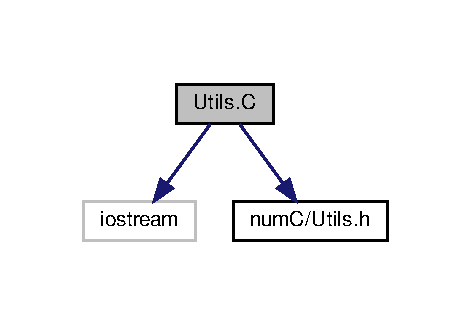
\includegraphics[width=226pt]{Utils_8C__incl}
\end{center}
\end{figure}
\subsubsection*{Functions}
\begin{DoxyCompactItemize}
\item 
void \hyperlink{Utils_8C_a3afdc4cf2cc3f040459fbd195e330f36}{readfile} (const char $\ast$fname, double $\ast$$\ast$x, double $\ast$$\ast$y, int n\+\_\+x, int n\+\_\+y)
\begin{DoxyCompactList}\small\item\em readfile \end{DoxyCompactList}\end{DoxyCompactItemize}


\subsubsection{Detailed Description}
File io utils. 



\subsubsection{Function Documentation}
\mbox{\Hypertarget{Utils_8C_a3afdc4cf2cc3f040459fbd195e330f36}\label{Utils_8C_a3afdc4cf2cc3f040459fbd195e330f36}} 
\index{Utils.\+C@{Utils.\+C}!readfile@{readfile}}
\index{readfile@{readfile}!Utils.\+C@{Utils.\+C}}
\paragraph{\texorpdfstring{readfile()}{readfile()}}
{\footnotesize\ttfamily void readfile (\begin{DoxyParamCaption}\item[{const char $\ast$}]{fname,  }\item[{double $\ast$$\ast$}]{x,  }\item[{double $\ast$$\ast$}]{y,  }\item[{int}]{n\+\_\+x = {\ttfamily 7},  }\item[{int}]{n\+\_\+y = {\ttfamily 200} }\end{DoxyParamCaption})}



readfile 

read file with specific format. To be generalized.

Parameters\+: 
\begin{DoxyParams}{Parameters}
{\em fname} & (const char$\ast$) file name to read \\
\hline
{\em x} & (double$\ast$$\ast$) data points \\
\hline
{\em y} & (double$\ast$$\ast$) data values \\
\hline
{\em n\+\_\+x} & (int) number of data points (default = 7) \\
\hline
{\em n\+\_\+y} & (int) number of data values (default = 200)\\
\hline
\end{DoxyParams}
Returns\+: \begin{DoxyReturn}{Returns}
void
\end{DoxyReturn}
Example\+:

readfile(data6, X, Y, 7, 200);

Tag\+: file io read file 

Definition at line 10 of file Utils.\+C.


\begin{DoxyCode}
10                                                                               \{
11   
12   FILE *data;
13   \textcolor{keywordtype}{char} buff[255];
14   std::string X = \textcolor{stringliteral}{"X"};
15   std::string data\_str = \textcolor{stringliteral}{"DATA"};
16 
17   \textcolor{keywordtype}{int} count=0;
18   \textcolor{keywordtype}{double} temp=0.;
19 
20   data = fopen(fname,\textcolor{stringliteral}{"r"});
21   
22   \textcolor{keywordflow}{while}(fscanf(data,\textcolor{stringliteral}{"%s"},buff)!=EOF)\{
23     \textcolor{keywordflow}{if}(!X.compare(buff))\{
24       \textcolor{keywordflow}{for}(\textcolor{keywordtype}{int} i=0;i<n\_x;i++)\{
25         fscanf(data, \textcolor{stringliteral}{"%lf"}, &temp);
26         *(*(x+i)+0) = temp;
27       \}
28       \textcolor{keywordflow}{continue};
29     \}
30     
31     \textcolor{keywordflow}{if}(!data\_str.compare(buff))\{
32       fscanf(data, \textcolor{stringliteral}{"%s"},buff);
33       \textcolor{keywordflow}{continue};
34     \}
35 
36     \textcolor{keywordflow}{for}(\textcolor{keywordtype}{int} i=0;i<n\_x;i++)\{
37       fscanf(data,\textcolor{stringliteral}{"%lf"},&temp);
38       *(*(y+i)+count) = temp;
39     \}
40     count++;
41   \}
42 
43   fclose(data);
44 
45   \textcolor{comment}{/*for(int i=0;i<7;i++) printf("%8.5f\(\backslash\)n",*(*(x+i)+0));}
46 \textcolor{comment}{  for(int i=0;i<7;i++)\{}
47 \textcolor{comment}{    for(int j=0;j<200;j++) printf("%8.5f\(\backslash\)t",*(*(y+i)+j));}
48 \textcolor{comment}{    printf("\(\backslash\)n");}
49 \textcolor{comment}{  \}*/}
50 \}
\end{DoxyCode}

\hypertarget{Utils_8h}{}\subsection{Utils.\+h File Reference}
\label{Utils_8h}\index{Utils.\+h@{Utils.\+h}}


File io uitls This functions are not compatible with Matrix\+\_\+gsl functions. This is compatible with \hyperlink{classMatrix}{Matrix} functions.  


This graph shows which files directly or indirectly include this file\+:
\nopagebreak
\begin{figure}[H]
\begin{center}
\leavevmode
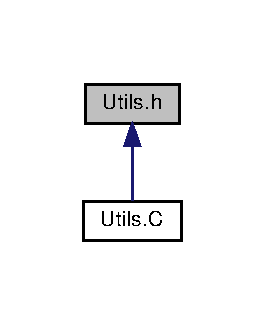
\includegraphics[width=127pt]{Utils_8h__dep__incl}
\end{center}
\end{figure}
\subsubsection*{Functions}
\begin{DoxyCompactItemize}
\item 
void \hyperlink{Utils_8h_a2798321f6823b728dda0aa7e343c6e52}{readfile} (const char $\ast$fname, double $\ast$$\ast$x, double $\ast$$\ast$y, int n\+\_\+x=7, int n\+\_\+y=200)
\begin{DoxyCompactList}\small\item\em readfile \end{DoxyCompactList}\end{DoxyCompactItemize}


\subsubsection{Detailed Description}
File io uitls This functions are not compatible with Matrix\+\_\+gsl functions. This is compatible with \hyperlink{classMatrix}{Matrix} functions. 

\begin{DoxyDate}{Date}
Nov 23, 2021 
\end{DoxyDate}
\begin{DoxyAuthor}{Author}
C J Park ~\newline
 \href{mailto:chanjure@snu.ac.kr}{\tt chanjure@snu.\+ac.\+kr} 
\end{DoxyAuthor}
\begin{DoxyRefDesc}{Bug}
\item[\hyperlink{bug__bug000004}{Bug}]No known bugs. \end{DoxyRefDesc}
\begin{DoxyVersion}{Version}
1.\+0 
\end{DoxyVersion}


\subsubsection{Function Documentation}
\mbox{\Hypertarget{Utils_8h_a2798321f6823b728dda0aa7e343c6e52}\label{Utils_8h_a2798321f6823b728dda0aa7e343c6e52}} 
\index{Utils.\+h@{Utils.\+h}!readfile@{readfile}}
\index{readfile@{readfile}!Utils.\+h@{Utils.\+h}}
\paragraph{\texorpdfstring{readfile()}{readfile()}}
{\footnotesize\ttfamily void readfile (\begin{DoxyParamCaption}\item[{const char $\ast$}]{fname,  }\item[{double $\ast$$\ast$}]{x,  }\item[{double $\ast$$\ast$}]{y,  }\item[{int}]{n\+\_\+x = {\ttfamily 7},  }\item[{int}]{n\+\_\+y = {\ttfamily 200} }\end{DoxyParamCaption})}



readfile 

read file with specific format. To be generalized.

Parameters\+: 
\begin{DoxyParams}{Parameters}
{\em fname} & (const char$\ast$) file name to read \\
\hline
{\em x} & (double$\ast$$\ast$) data points \\
\hline
{\em y} & (double$\ast$$\ast$) data values \\
\hline
{\em n\+\_\+x} & (int) number of data points (default = 7) \\
\hline
{\em n\+\_\+y} & (int) number of data values (default = 200)\\
\hline
\end{DoxyParams}
Returns\+: \begin{DoxyReturn}{Returns}
void
\end{DoxyReturn}
Example\+:

readfile(data6, X, Y, 7, 200);

Tag\+: file io read file 

Definition at line 5 of file Utils.\+C.


\begin{DoxyCode}
5                                                                               \{
6   
7   FILE *data;
8   \textcolor{keywordtype}{char} buff[255];
9   std::string X = \textcolor{stringliteral}{"X"};
10   std::string data\_str = \textcolor{stringliteral}{"DATA"};
11 
12   \textcolor{keywordtype}{int} count=0;
13   \textcolor{keywordtype}{double} temp=0.;
14 
15   data = fopen(fname,\textcolor{stringliteral}{"r"});
16   
17   \textcolor{keywordflow}{while}(fscanf(data,\textcolor{stringliteral}{"%s"},buff)!=EOF)\{
18     \textcolor{keywordflow}{if}(!X.compare(buff))\{
19       \textcolor{keywordflow}{for}(\textcolor{keywordtype}{int} i=0;i<n\_x;i++)\{
20         fscanf(data, \textcolor{stringliteral}{"%lf"}, &temp);
21         *(*(x+i)+0) = temp;
22       \}
23       \textcolor{keywordflow}{continue};
24     \}
25     
26     \textcolor{keywordflow}{if}(!data\_str.compare(buff))\{
27       fscanf(data, \textcolor{stringliteral}{"%s"},buff);
28       \textcolor{keywordflow}{continue};
29     \}
30 
31     \textcolor{keywordflow}{for}(\textcolor{keywordtype}{int} i=0;i<n\_x;i++)\{
32       fscanf(data,\textcolor{stringliteral}{"%lf"},&temp);
33       *(*(y+i)+count) = temp;
34     \}
35     count++;
36   \}
37 
38   fclose(data);
39 
40   \textcolor{comment}{/*for(int i=0;i<7;i++) printf("%8.5f\(\backslash\)n",*(*(x+i)+0));}
41 \textcolor{comment}{  for(int i=0;i<7;i++)\{}
42 \textcolor{comment}{    for(int j=0;j<200;j++) printf("%8.5f\(\backslash\)t",*(*(y+i)+j));}
43 \textcolor{comment}{    printf("\(\backslash\)n");}
44 \textcolor{comment}{  \}*/}
45 \}
\end{DoxyCode}

%--- End generated contents ---

% Index
\newpage
\phantomsection
\clearemptydoublepage
\addcontentsline{toc}{section}{Index}
\printindex

\end{document}
